%%%%%%%%%%%%%%%%%%%%%%%%%%%%%%%%%%%%%%%%%
% University Assignment Title Page 
% LaTeX Template
% Version 1.0 (27/12/12)
%
% This template has been downloaded from:
% http://www.LaTeXTemplates.com
%
% Original author:
% WikiBooks (http://en.wikibooks.org/wiki/LaTeX/Title_Creation)
%
% License:
% CC BY-NC-SA 3.0 (http://creativecommons.org/licenses/by-nc-sa/3.0/)
% 
% Instructions for using this template:
% This title page is capable of being compiled as is. This is not useful for 
% including it in another document. To do this, you have two options: 
%
% 1) Copy/paste everything between \begin{document} and \end{document} 
% starting at \begin{titlepage} and paste this into another LaTeX file where you 
% want your title page.
% OR
% 2) Remove everything outside the \begin{titlepage} and \end{titlepage} and 
% move this file to the same directory as the LaTeX file you wish to add it to. 
% Then add %%%%%%%%%%%%%%%%%%%%%%%%%%%%%%%%%%%%%%%%%
% University Assignment Title Page 
% LaTeX Template
% Version 1.0 (27/12/12)
%
% This template has been downloaded from:
% http://www.LaTeXTemplates.com
%
% Original author:
% WikiBooks (http://en.wikibooks.org/wiki/LaTeX/Title_Creation)
%
% License:
% CC BY-NC-SA 3.0 (http://creativecommons.org/licenses/by-nc-sa/3.0/)
% 
% Instructions for using this template:
% This title page is capable of being compiled as is. This is not useful for 
% including it in another document. To do this, you have two options: 
%
% 1) Copy/paste everything between \begin{document} and \end{document} 
% starting at \begin{titlepage} and paste this into another LaTeX file where you 
% want your title page.
% OR
% 2) Remove everything outside the \begin{titlepage} and \end{titlepage} and 
% move this file to the same directory as the LaTeX file you wish to add it to. 
% Then add %%%%%%%%%%%%%%%%%%%%%%%%%%%%%%%%%%%%%%%%%
% University Assignment Title Page 
% LaTeX Template
% Version 1.0 (27/12/12)
%
% This template has been downloaded from:
% http://www.LaTeXTemplates.com
%
% Original author:
% WikiBooks (http://en.wikibooks.org/wiki/LaTeX/Title_Creation)
%
% License:
% CC BY-NC-SA 3.0 (http://creativecommons.org/licenses/by-nc-sa/3.0/)
% 
% Instructions for using this template:
% This title page is capable of being compiled as is. This is not useful for 
% including it in another document. To do this, you have two options: 
%
% 1) Copy/paste everything between \begin{document} and \end{document} 
% starting at \begin{titlepage} and paste this into another LaTeX file where you 
% want your title page.
% OR
% 2) Remove everything outside the \begin{titlepage} and \end{titlepage} and 
% move this file to the same directory as the LaTeX file you wish to add it to. 
% Then add %%%%%%%%%%%%%%%%%%%%%%%%%%%%%%%%%%%%%%%%%
% University Assignment Title Page 
% LaTeX Template
% Version 1.0 (27/12/12)
%
% This template has been downloaded from:
% http://www.LaTeXTemplates.com
%
% Original author:
% WikiBooks (http://en.wikibooks.org/wiki/LaTeX/Title_Creation)
%
% License:
% CC BY-NC-SA 3.0 (http://creativecommons.org/licenses/by-nc-sa/3.0/)
% 
% Instructions for using this template:
% This title page is capable of being compiled as is. This is not useful for 
% including it in another document. To do this, you have two options: 
%
% 1) Copy/paste everything between \begin{document} and \end{document} 
% starting at \begin{titlepage} and paste this into another LaTeX file where you 
% want your title page.
% OR
% 2) Remove everything outside the \begin{titlepage} and \end{titlepage} and 
% move this file to the same directory as the LaTeX file you wish to add it to. 
% Then add \input{./title_page_1.tex} to your LaTeX file where you want your

% title page.
%
%%%%%%%%%%%%%%%%%%%%%%%%%%%%%%%%%%%%%%%%%
%\title{Title page with logo}
%----------------------------------------------------------------------------------------
%	PACKAGES AND OTHER DOCUMENT CONFIGURATIONS
%----------------------------------------------------------------------------------------

\documentclass[12pt]{article}
\usepackage[spanish]{babel}
\usepackage[utf8x]{inputenc}
\usepackage{amsmath}
\usepackage{graphicx}
\usepackage[colorinlistoftodos]{todonotes}

\begin{document}

\begin{titlepage}

\newcommand{\HRule}{\rule{\linewidth}{0.5mm}} % Defines a new command for the horizontal lines, change thickness here

\center % Center everything on the page
 
%----------------------------------------------------------------------------------------
%	HEADING SECTIONS
%----------------------------------------------------------------------------------------

\textsc{\LARGE Universidad de Antioquia}\\[1.5cm] % Name of your university/college
\textsc{\Large Facultad de Ciencias Exactas y Naturales}\\[0.5cm]
% Major heading such as course name
\textsc{\Large Instituto de Física}\\[0.5cm]
\textsc{\large Proyecto de Maestría}\\[0.5cm] % Minor heading such as course title

%----------------------------------------------------------------------------------------
%	TITLE SECTION
%----------------------------------------------------------------------------------------

\HRule \\[0.4cm]
{ \huge \bfseries High Level Trigger studies for the detection of dark matter in models with vector like fermions using the CMS detector in the LHC}\\[0.4cm] % Title of your document
\HRule \\[1.5cm]
 
%----------------------------------------------------------------------------------------
%	AUTHOR SECTION
%----------------------------------------------------------------------------------------

\begin{minipage}{0.4\textwidth}
\begin{flushleft} \large
\emph{Autor:}\\
Diego Barón \textsc{} % Your name
\end{flushleft}
\end{minipage}
~
\begin{minipage}{0.4\textwidth}
\begin{flushright} \large
\emph{Asesor:} \\
Nelson Vanegas \textsc{} % Supervisor's Name
\end{flushright}
\end{minipage}\\[1.2cm]

% If you don't want a supervisor, uncomment the two lines below and remove the section above
%\Large \emph{Author:}\\
%John \textsc{Smith}\\[3cm] % Your name

%----------------------------------------------------------------------------------------
%	DATE SECTION
%----------------------------------------------------------------------------------------

{\large \today}\\[0.7cm] % Date, change the \today to a set date if you want to be precise

%----------------------------------------------------------------------------------------
%	LOGO SECTION
%----------------------------------------------------------------------------------------


\includegraphics[width=2.8cm]{udea_fcen.jpg}\\[4cm] % Include a department/university logo - this will requireu the graphicx packag0.7
 
%----------------------------------------------------------------------------------------

\vfill % Fill the rest of the page with whitespace

\end{titlepage}

\tableofcontents % indice de contenidos

\cleardoublepage





\section{Generalidades del proyecto.}

\textbf{Titulo del proyecto:}\\
High Level Trigger studies for the detection of dark matter in models with vector like fermions using the CMS detector in the LHC
\\

\textbf{Línea de investigación:}\\
Física de partículas experimental.
\\

\textbf{Duración:}\\
Dos años.
\\

\textbf{Lugar de ejecución:}\\
Universidad de Antioquia.
\\

\textbf{Equipo de investigación:}\\
\emph{Diego Barón}: Estudiante de maestría.
\emph{Nelson Vanegas}: Asesor, director proyecto UdeA-CMS.
\emph{Jose David Ruíz}: Coasesor, investigador en CMS.
\\

\textbf{Resumen ejecutivo:}\\
En este trabajo se presenta la propuesta de trabajo del estudiante de maestría Diego Barón. Desde 1930 gracias a las observaciones de las curvas de rotacion de las estrellas en las galaxias se plantea la existencia de la materia oscura 


\newpage























\section{Marco conceptual.}
El problema de la materia oscura (DM) es quizás el problema más viejo de la física de partículas, que aún no ha sido satisfactoriamente resuelto, desde 1930 gracias a las observaciones independientes de Lundmark y Zwicky se sabe que el contenido de materia de las galaxias debe ser mayor al que aporta la materia bariónica, en sus experimentos esto se expresaba como el hecho de que las velocidades orbitales del gas y de las estrellas mantiene una tendencia constante respecto a la distancia al centro de la galaxia, en contraposción con lo esperado: que la velocidad decrezca como una función de la distancia. Esto se puede ver en la figura 1.
\\
\\
\begin{figure}
\centering
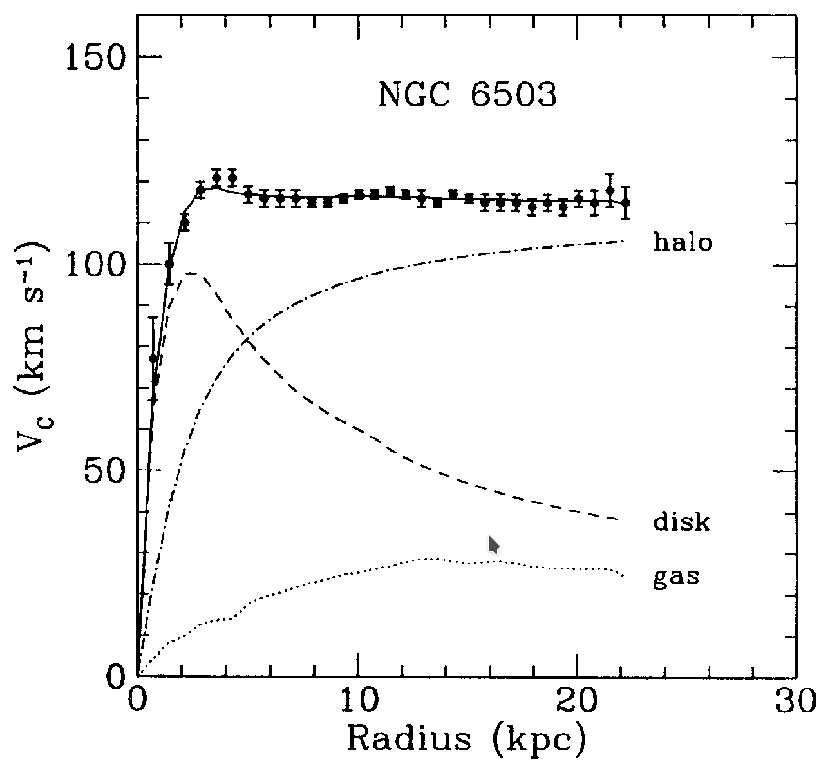
\includegraphics[width=12cm]{F1.png}
\caption{\label{fig:frog} Curva de rotacion galáctica para NGC 6503, vemos el perfil de masa del disco y del gas y el perfil de materia oscura necesario para ajustar los datos.}
\end{figure}
Vamos a describir como se puede utilizar un detector como el CMS en el LHC para hacer busquedas de posibles candidatos a DM, poniendo especial atención en el High Level Trigger (HLT).


\label{sec:examples}

\subsection{CMS en el LHC.}

El Gran Colisionador de Hadrones (LHC) es el acelerador de partículas más grande y energético operado actualmente por la Organización Europea para la Investigación Nuclear (CERN), el LHC usa el mismo tunel de 27 km, cavado en promedio a 100 m de profundidad, del antiguo Gran Colisionador Electrón-Positrón (LEP). EL LHC es capaz de colisionar protones e iones de Plomo con una energía por haz de 7 TeV, sin embargo a día de hoy se hace a 6.5 TeV.
\\

En el LHC están ubicados 4 experimentos principales: LHC-b, ALICE, ATLAS y CMS. Estos últimos dos son detectores de proposito general, es decir, fueron diseñados para detectar señales de nueva física en estados finales de partículas como electrones, fotones, muones y jets de hadrones. El LHC esta dividido en dos partes: la cadena de aceleración y el anillo principal. En la cadena de aceleración los protones son extraídos y pasados por una serie de aceleradores que los llevan hasta una energía de 450 GeV, momento en que son inyectados en el anillo principal. Este está compuesto de dos anillos que llevan los protones en direcciones opuestas,los anillos están construidos por 2090 imanes de 15 m, enfriados a 1.9 K y con un vacío de $10^{-9}$mbar, cada uno capaz de producir un campo magnético de 8,33 T. Además de estos imanes dipolares, el LHC también cuenta con 520 cuadrupolos, 2464 sextupolos y 1232 octupolos usados para colimar el haz. [1]
\\
\\

El Solenoide Compacto de Muones (CMS) es, en tamaño, el segundo experimento más grande del LHC despues de ATLAS, debe su nombre (solenoide compacto) a que varios de los sistemas de detección se encuentran dentro del su gran imán superconductor, capaz de producir un campo magnético uniforme en su interior de 3.8 T y (de muones) debido a que posee un sistema de detección de muones muy preciso y eficiente. CMS es un detector con forma cilíndrica, mide aproximadamente 30 m de largo por 15 m de diámetro, pesa 14000 Ton (esto lo convierte en el experimento más pesado del LHC) y la colaboración se compone de aproximadamente 3500 personas de 182 institutos de física en 41 países. Una representación tres dimensional del detector se puede ver en la figura 2.
\\
\\
\begin{figure}
\centering
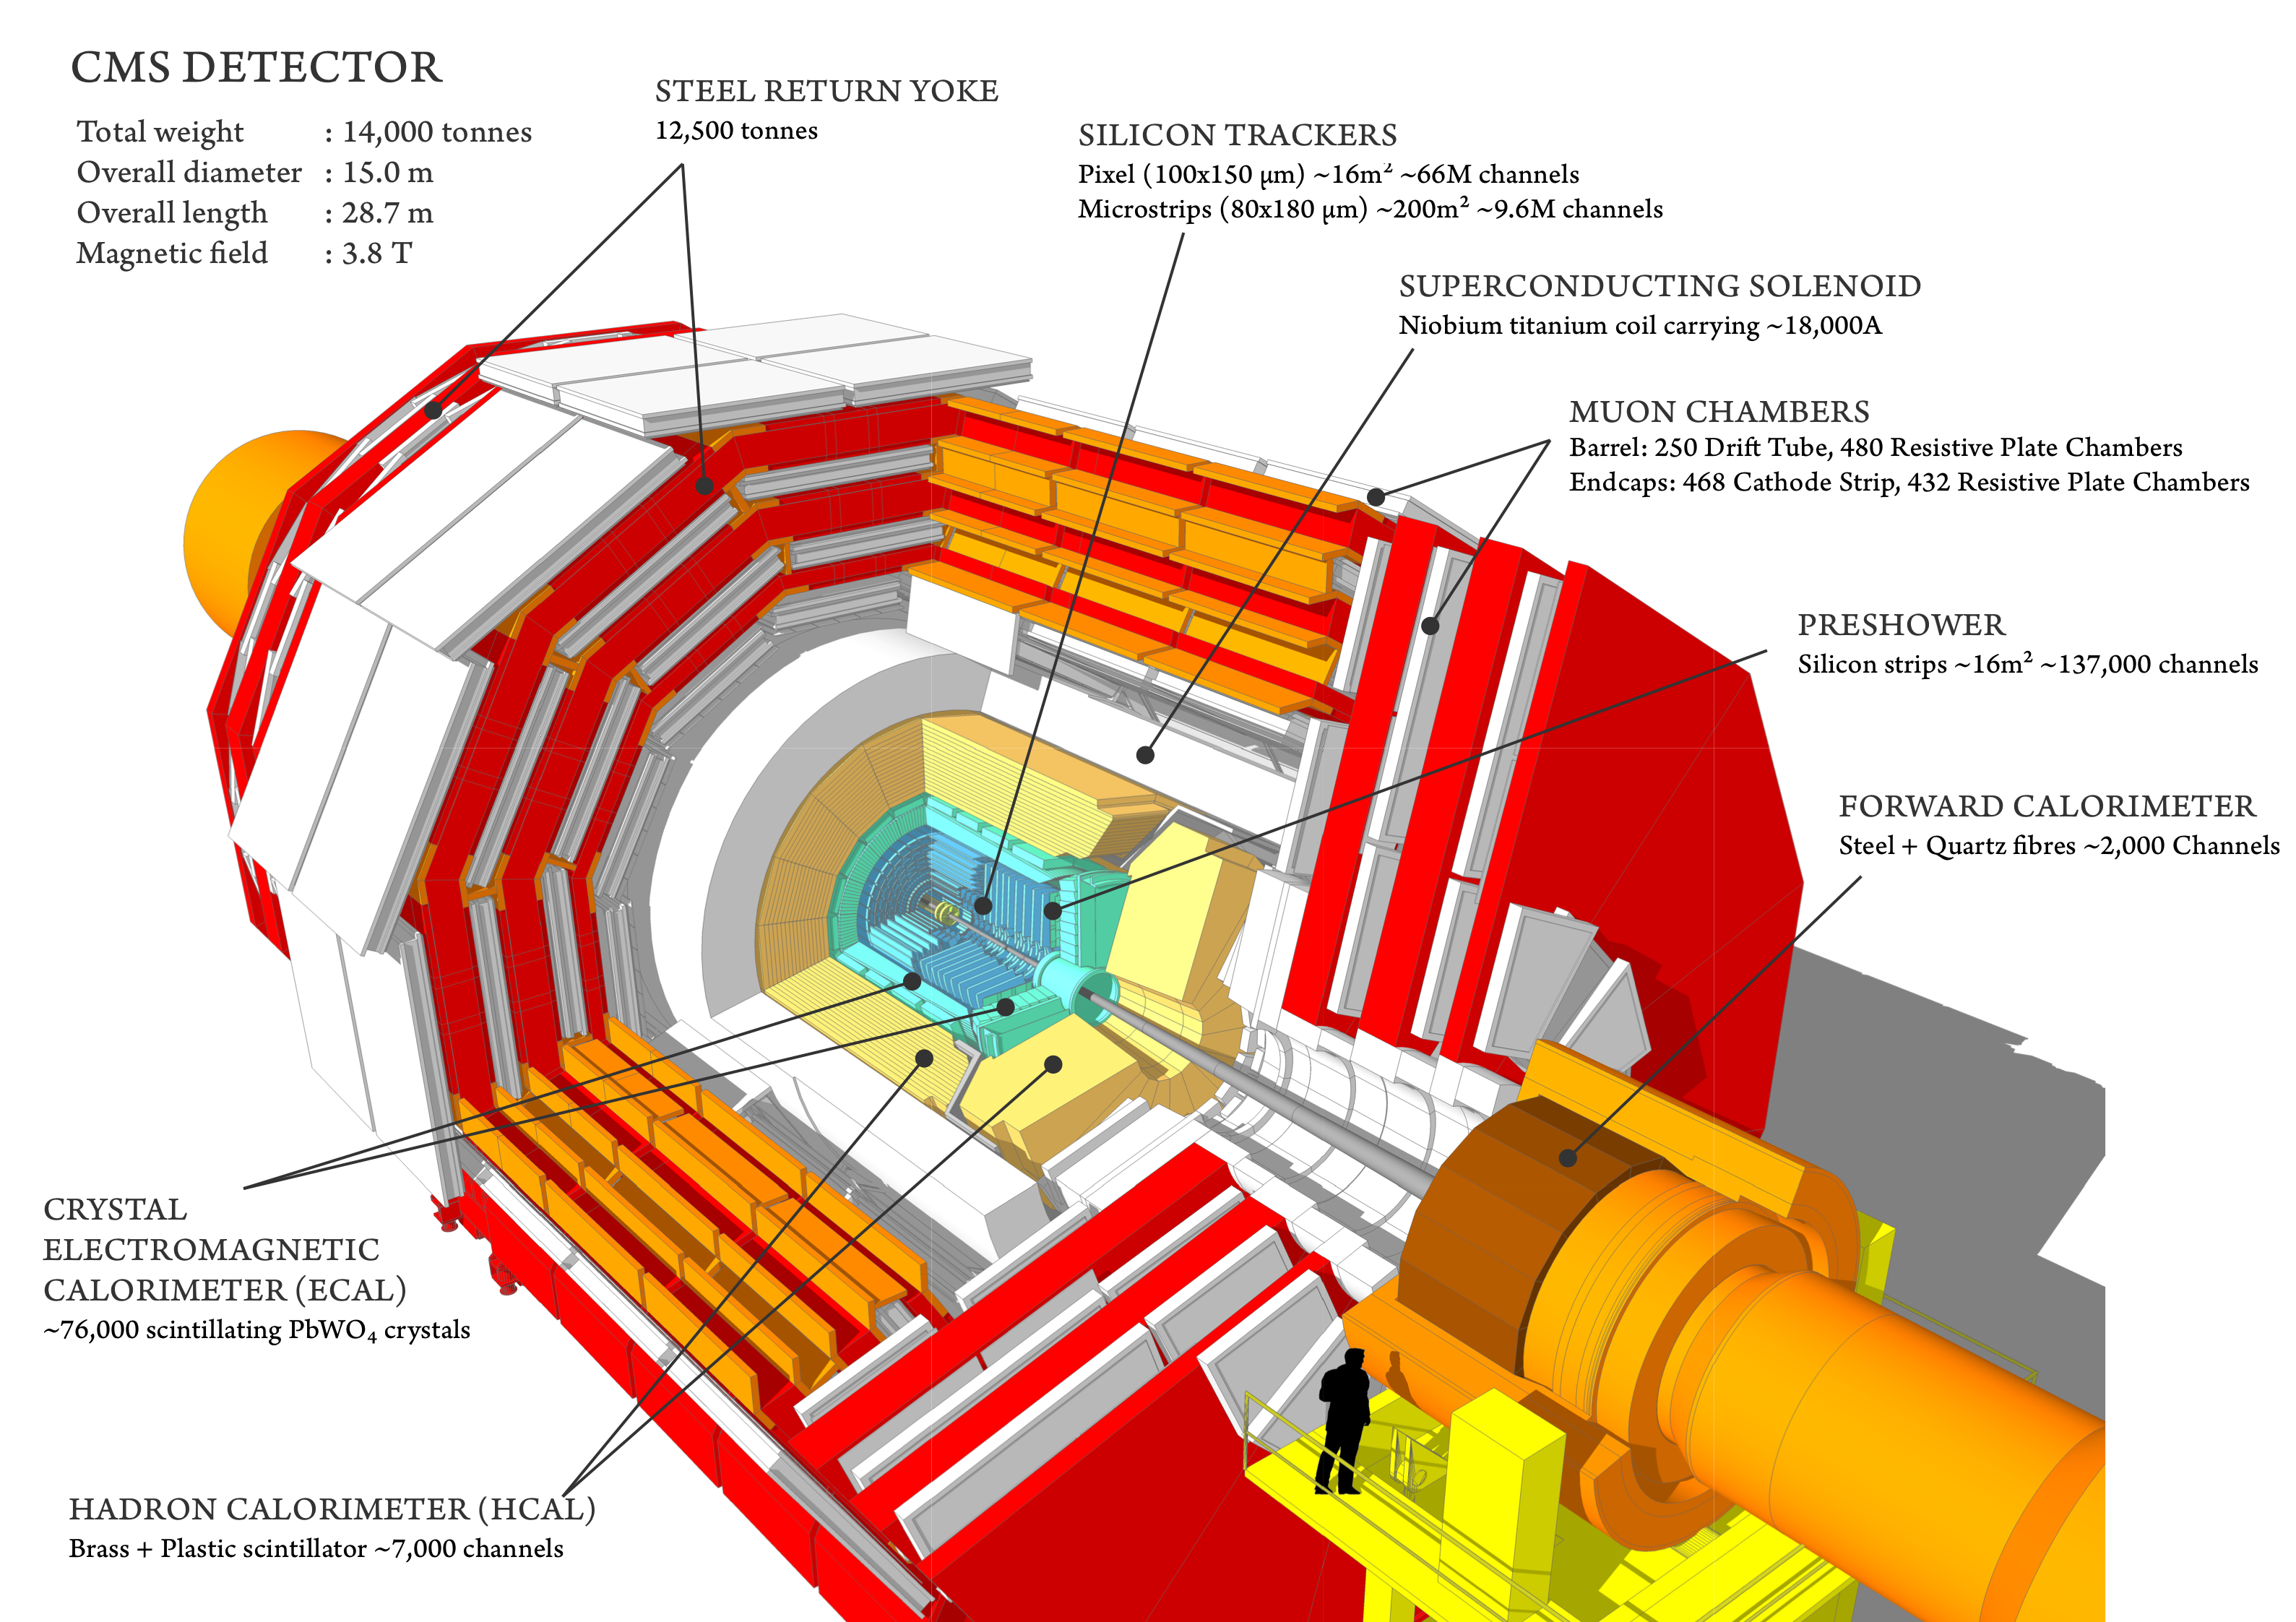
\includegraphics[width=15cm]{F2.png}
\caption{\label{fig:frog} Diseño interno del detector CMS.}
\end{figure}


El imán del CMS tiene 13 m de largo y 6 m de diametro, es capaz de generar un campo magnético uniforme de 4 T en su interior y está construido por 4 capas de espiras de NbTi a 4.45K para que se alcance el estado superconductor, este imán está rodeado por 5 barriles y 3 discos de hierro que tienen el objetivo de devolver el campo magnético generando un campo exterior de 2 T,  esta configuración de campos magnéticos es responsable de curvar las trayectorias de las partículas cargadas.
\\
\\

Dentro del solenoide se encuentra el Tracker System, un sistema de detección diseñado con dos tecnologías: Pixeles y tiras de silicio, está diseñado para identificar los vertices de las colisiones con una precisión de 9 $\mu$m y una eficiencia del 98\% (que se degrada con la luminosidad integrada), cuando una partícula cargada pasa se crean pares electrón-hueco en el material y esto genera una señal eléctrica que luego es amplificada, este sistema fue construido para ser bastante resistente a la radiación y se espera que dure 10 años.
\\
\\
Luego de este sistema se encuentra el calorímetro electromagnético (ECAL), este fue construido para detener electrones y fotones y medir su energía, el sistema está compuesto por cristales de tungstato de plomo, el cual fue escogido por su corta profundidad de radiación, alta densidad y rápido centelleo (25 ns), la unica desventaja del mismo es su alta sensibilidad de respuesta a la temperatura (2\%/C). Los cristales van perdiendo transparencia con la luminosidad integrada y por tanto esta tiene que ser corregida constantemente por un sistema de láser. El sistema cuenta con 61200 cristales en el barril y 7324 en las tapas del calorímetro.
\\
\\
Para detener y detectar los jets hadrónicos se diseñó el calorímetro hadrónico (HCAL), de este sistema cierta parte se encuentra dentro del solenoide (Hadron Endcap Calorimeter y Hadron Barrel Calorimeter) y fuera están el Outer Calorimeter y el Hadron Forward Calorimeter (estos permiten extender el rango angular de detección), los calorímetros tienen el objetivo de detectar los hadrones y lo hacen de la siguiente manera: el sistema tiene intercalados placas de acero con cristales centelladores, las placas de acero generan las duchas de hadrones y cuando estos pasan por los centelladores, la luz generada es convertida en corrientes eléctricas por fotodiodos híbridos (HPDs), estas corrientes permiten medir la energía de los hadrones. Es importante mencionar que debido a la posición del Forward Calorimeter, este recibe mucha radiación comparado a los otros calorìmetros hadrónicos y esto es debido a que está en la dirección del haz incidente y por tanto, los centelladores fueron construidos de un material centellador más resistente a la radiación como lo es el cuarzo.
\\
\\
Finalmente en la parte más externa del detector están ubicados los detectores de muones, esto se debe a que estas partículas tienen un gran poder de penetración. Las cámaras de deteccion están hechas de 3 tecnologías diferentes: Drift Tube Chambers (DT), Cathode Strip Chambers(CSC) y Resistive Plate Chambers (RPC), sin embargo las 3 están basadas en la ionización de gases: al paso de partículas cargadas se generan corrientes de deriva. En la figura 3 se muestra una recreación a un corte transversal del detector.

\begin{figure}
\centering
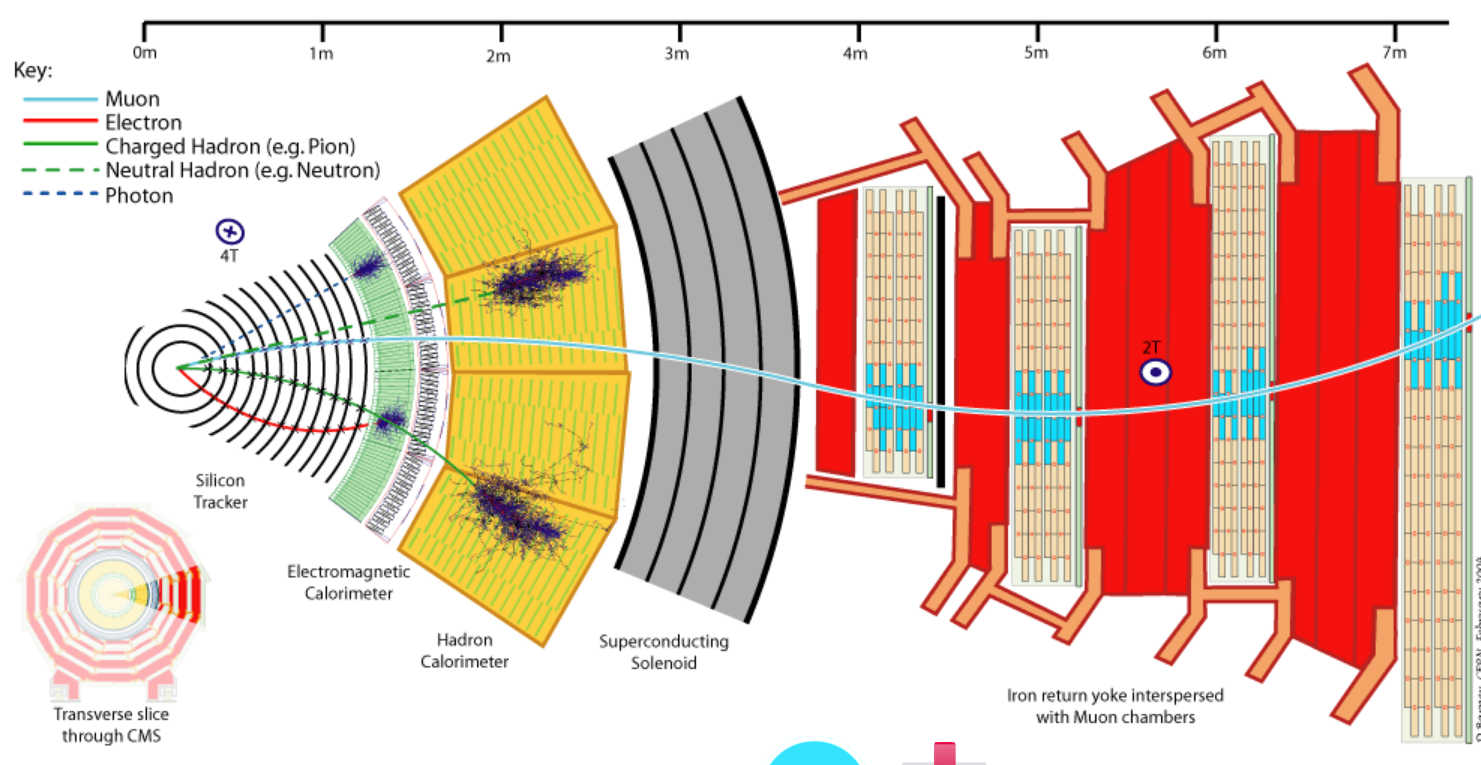
\includegraphics[width=15cm]{F3.png}
\caption{\label{fig:frog} Corte transversal del detector CMS.}
\end{figure}

\subsection{Sistema de Trigger.}

El LHC fue diseñado para tomar los datos de cada colisión que ocurre, cada una está separada en el tiempo por 25 ns, esto produce un flujo de datos de 1 PB/s (PB=Petabyte). Por tanto debe hacerse una selección de eventos en tiempo real, el sistema encargado de hacer esto recibe el nombre de Trigger System y lleva a cabo esta tarea en 2 fases. [2]
\\
\\
La primera de ellas es el Level 1 Trigger (L1), este es un proceso basado en Hardware construido especificamente para analizar los datos provenientes de los sistemas de detección y escoger los eventos más interesantes: aquellos que contienen partículas con gran momento transverso o por ejemplo con combinaciones raras de estados finales. Este filtro reduce el flujo de datos en 2 ordenes de magnitud y dispone de 3.2 $\mu$s para decidir, esto hace que la memoria de almacenamiento deba ser suficiente para guardar los datos de 128  colisiones.
\\
\\
La segunda fase de la selección se conoce como High Level Trigger (HLT) y es un proceso basado en software, una serie de algoritmos corren en granjas de varios miles de procesadores, los códigos han sido previamente implementados con el objetivo de realizar búsquedas predeterminadas y analizan los datos que salen de L1, el tiempo de decisión de este sistema es de aproximadamente 100 ms, al finalizar la selección el flujo original de datos ha sido reducido por un factor de 5 ordenes de magnitud.

\subsection{Materia oscura en colisionadores.}

El modelo estándar de la cosmología predice que solo conocemos como se comporta el 5\% del contenido de materia del universo (materia bariónica), el restante 95\% es: materia oscura (26\%) y energía oscura (69\%) [3], las evidencias de la existencia de materia oscura son variadas y contundentes: lentes gravitacionales, el cúmulo bala, la radiación cósmica de fondo y la estababilidad del gas caliente en clusters de galaxias son algunas de ellas. [4] 
\\
\\
Hace 20 años algunas propuestas a candidatos de materia oscura incluían los MACHOS (Massive compact halo objects), que consisten de objetos astrofísicos muy tenues para ser detectados, por ejemplo: agujeros negros, estrellas de neutrones, enanas blancas, etc. Sin embargo experimentos recientes descartan esta posibilidad y por tanto nos dejan solo con los candidatos no bariónicos como posibles explicaciones. [5,6]
\\
\\
Los candidatos más populares actualmente son los WIMPS (weakly interacting massive particles) y los Axiones, ambas son partículas que surgen como propuesta a la solución de otros problemas en física de partículas (SUSY y CP Fuerte respectivamente) y por esto son tan populares, se sabe que la materia oscura no puede ser caliente, es decir, tener velocidades relativistas, debido a que esto implicaría que el universo fuera más homogéneo de lo que es y tampoco puede interactuar eléctricamente. Otros candidatos para materia oscura surgen de modelos más sencillos como el modelo del doblete inerte y pueden ser detectados en aceleradores como muestran recientes trabajos. [7,8] Esta busqueda en particular se basa en la fusión de bosones vectoriales (VBF) ya que el candidato a materia oscura $H^0$ tiene carga débil. En la figura 4 podemos ver los procesos que contribuyen en este tipo de busquedas, como vemos de los estados finales en los diagramas (jets que se detectan y el candidato de materia oscura escapa), las busquedas se basan en energía transversa faltante (MET) asociada a procesos con dos jets con energía transversa $E_T$ alta y detectados en hemisferios diferentes.
\begin{figure}
	\centering
	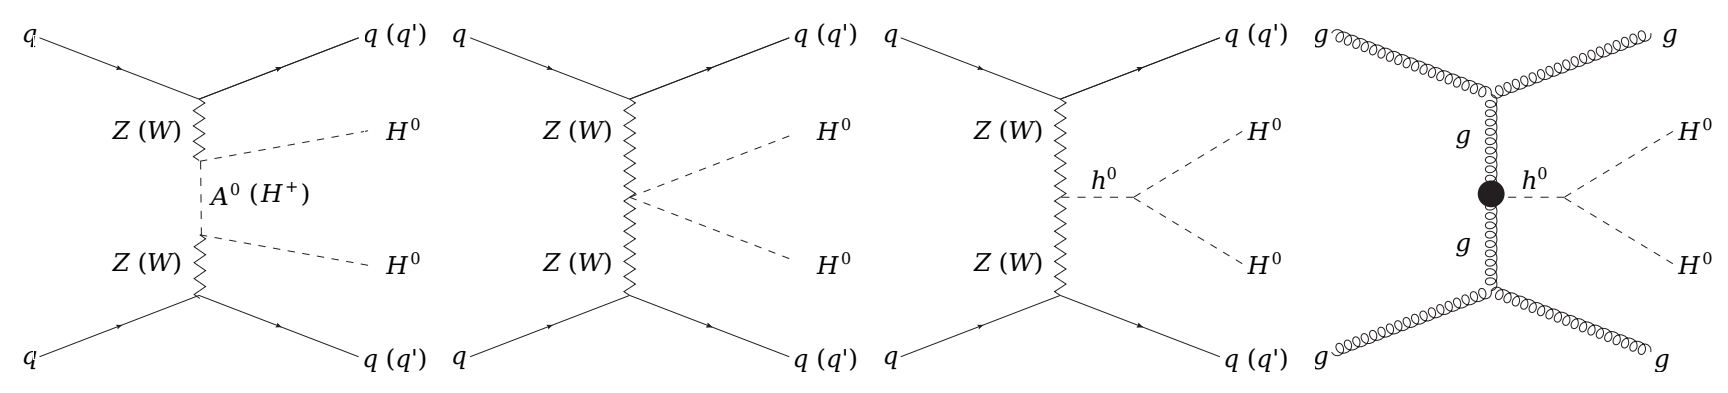
\includegraphics[width=15cm]{F4.png}
	\caption{\label{fig:frog} Diagramas de Feynman que contribuyen a pp$\rightarrow H^0H^0 jj$. El punto en la cuarta figura denota el acople entre el Higgs del modelo estándar y los gluones.}
\end{figure}
\\
\\
Las busquedas en aceleradores como el LHC se basan en la busqueda de estados finales de partículas del modelo estándar con energía transversa faltante [7], de esta manera sabríamos que la partícula de materia oscura vivió lo suficiente como para escapar del detector sin decaer, sin embargo esto no dejaría claro que tan estable es la misma para ser materia oscura y por tanto es necesario complementar la información con experimentos astrofísicos. [9]
\newpage
\section{Problema y pregunta de investigación.}

	Conforme a lo establecido en las secciones anteriores, podemos ver que el problema de encontrar la materia oscura debe resolverse, en parte, mediante la busqueda de la misma en colisionadores, ya hemos visto que modelos como [7,8] motivan busquedas en experimentos como LHC, sin embargo, debido a la cantidad de datos que toman detectores como CMS se deben idear filtros que nos dejen con la información que consideramos relevante a la hora de realizar las busquedas, por tanto nuestra idea es responder: \textbf{¿Qué Hight Level Trigger para el experimento CMS del CERN es pertinente para su uso en el estudio de señales de materia oscura en el detector?}


\newpage
\section{Objetivos y cronograma.}


\subsection{Objetivo general.}

Desarrollar un Hight Level Trigger (HLT) para el experimento CMS del CERN pertinente para su uso en el estudio de señales de materia oscura en el detector.

\subsection{Objetivos específicos.}

\begin{itemize}
	\item Revisión constante de bibliografía.
	\item Estudiar la herramienta de construcción de HLT de CMS.
	\item Estudio del modelo que desea ponerse a prueba, estudianto la señal que quiere detectarse y sus background.
	\item Construcción del HLT usando la herramienta de CMS.
	\item Estudiar la eficiencia y otras características de dicho HLT y proponerlo.
	\item Aplicar el HLT al menos a un modelo específico, un ejemplo podrían ser los modelos [7,8].
\end{itemize}


\subsection{Cronograma.}

\begin{table}[h]
	\centering
	
	\label{my-label}
	\begin{tabular}{|c|c|c|c|c|c|c|c|c|}
		\hline
		Trimestre                              & 2017-3 & 2017-4 & 2018-1 & 2018-2 & 2018-3 & 2018-4 & 2019-1 & 2019-2 \\ \hline
		Revisión de bibliografía.              & *      & *      & *      & *      & *      & *      & *      &        \\ \hline
		Estudio herramienta HLT de CMS.        &        & *      & *      & *      &        &        &        &        \\ \hline
		Estudio fenomenológico.                &        &        & *      & *      &        &        &        &        \\ \hline
		Construcción del HLT                   &        &        &        & *      & *      & *      &        &        \\ \hline
		Estudio de eficiencia.                 &        &        &        &        & *      & *      &        &        \\ \hline
		Aplicar el HLT a un modelo específico. &        &        &        &        &        & *      & *      &        \\ \hline
		Redacción tesis.                       &        &        &        &        &        &        & *      & *      \\ \hline
	\end{tabular}
\end{table}
\section{Infraestructura y recursos.}

\section{Bibliografía.}

[1] Search for a vector-like quark T decaying into top+Higgs in single production mode in full hadronic final state using CMS data collected at 8 TeV, José David Ruiz.
\vspace{0.5cm}

[2] The CMS trigger system, CMS collaboration.

\vspace{0.5cm}

[3] Planck Collaboration, P. A. R. Ade et al., Planck 2015 results. XIII. Cosmo-
logical parameters, arXiv:1502.01589, Astron. Astrophys. 594, A13 (2016).

\vspace{0.5cm}

[4] Status of dark matter in the universe, Katherine Freese.

\vspace{0.5cm}

[5] LIMITS ON STELLAR OBJECTS AS THE DARK MATTER OF OUR HALO: NONBARYONICDARK MATTER SEEMS TO BE REQUIRED, Katherine Freese et al.

\vspace{0.5cm}

[6] SChemical Abundance Constraints on White Dwarfs as Halo Dark Matter, Brian D. Fields et al.

\vspace{0.5cm}

[7] Vector Boson Fusion in the Inert Doublet Model, Bhaskar Dutta, Guillermo Palacio, Diego Restrepo, José D. Ruiz.

\vspace{0.5cm}

[8] Andres G. Delannoy et al., “Probing Dark Matter at the LHC using Vector Boson Fusion
Processes,” Phys. Rev. Lett. 111, 061801 (2013).

\vspace{0.5cm}

[9] Review of Dark Matter searches at colliders, Sarah Alam Malik.


\end{document} to your LaTeX file where you want your

% title page.
%
%%%%%%%%%%%%%%%%%%%%%%%%%%%%%%%%%%%%%%%%%
%\title{Title page with logo}
%----------------------------------------------------------------------------------------
%	PACKAGES AND OTHER DOCUMENT CONFIGURATIONS
%----------------------------------------------------------------------------------------

\documentclass[12pt]{article}
\usepackage[spanish]{babel}
\usepackage[utf8x]{inputenc}
\usepackage{amsmath}
\usepackage{graphicx}
\usepackage[colorinlistoftodos]{todonotes}

\begin{document}

\begin{titlepage}

\newcommand{\HRule}{\rule{\linewidth}{0.5mm}} % Defines a new command for the horizontal lines, change thickness here

\center % Center everything on the page
 
%----------------------------------------------------------------------------------------
%	HEADING SECTIONS
%----------------------------------------------------------------------------------------

\textsc{\LARGE Universidad de Antioquia}\\[1.5cm] % Name of your university/college
\textsc{\Large Facultad de Ciencias Exactas y Naturales}\\[0.5cm]
% Major heading such as course name
\textsc{\Large Instituto de Física}\\[0.5cm]
\textsc{\large Proyecto de Maestría}\\[0.5cm] % Minor heading such as course title

%----------------------------------------------------------------------------------------
%	TITLE SECTION
%----------------------------------------------------------------------------------------

\HRule \\[0.4cm]
{ \huge \bfseries High Level Trigger studies for the detection of dark matter in models with vector like fermions using the CMS detector in the LHC}\\[0.4cm] % Title of your document
\HRule \\[1.5cm]
 
%----------------------------------------------------------------------------------------
%	AUTHOR SECTION
%----------------------------------------------------------------------------------------

\begin{minipage}{0.4\textwidth}
\begin{flushleft} \large
\emph{Autor:}\\
Diego Barón \textsc{} % Your name
\end{flushleft}
\end{minipage}
~
\begin{minipage}{0.4\textwidth}
\begin{flushright} \large
\emph{Asesor:} \\
Nelson Vanegas \textsc{} % Supervisor's Name
\end{flushright}
\end{minipage}\\[1.2cm]

% If you don't want a supervisor, uncomment the two lines below and remove the section above
%\Large \emph{Author:}\\
%John \textsc{Smith}\\[3cm] % Your name

%----------------------------------------------------------------------------------------
%	DATE SECTION
%----------------------------------------------------------------------------------------

{\large \today}\\[0.7cm] % Date, change the \today to a set date if you want to be precise

%----------------------------------------------------------------------------------------
%	LOGO SECTION
%----------------------------------------------------------------------------------------


\includegraphics[width=2.8cm]{udea_fcen.jpg}\\[4cm] % Include a department/university logo - this will requireu the graphicx packag0.7
 
%----------------------------------------------------------------------------------------

\vfill % Fill the rest of the page with whitespace

\end{titlepage}

\tableofcontents % indice de contenidos

\cleardoublepage





\section{Generalidades del proyecto.}

\textbf{Titulo del proyecto:}\\
High Level Trigger studies for the detection of dark matter in models with vector like fermions using the CMS detector in the LHC
\\

\textbf{Línea de investigación:}\\
Física de partículas experimental.
\\

\textbf{Duración:}\\
Dos años.
\\

\textbf{Lugar de ejecución:}\\
Universidad de Antioquia.
\\

\textbf{Equipo de investigación:}\\
\emph{Diego Barón}: Estudiante de maestría.
\emph{Nelson Vanegas}: Asesor, director proyecto UdeA-CMS.
\emph{Jose David Ruíz}: Coasesor, investigador en CMS.
\\

\textbf{Resumen ejecutivo:}\\
En este trabajo se presenta la propuesta de trabajo del estudiante de maestría Diego Barón. Desde 1930 gracias a las observaciones de las curvas de rotacion de las estrellas en las galaxias se plantea la existencia de la materia oscura 


\newpage























\section{Marco conceptual.}
El problema de la materia oscura (DM) es quizás el problema más viejo de la física de partículas, que aún no ha sido satisfactoriamente resuelto, desde 1930 gracias a las observaciones independientes de Lundmark y Zwicky se sabe que el contenido de materia de las galaxias debe ser mayor al que aporta la materia bariónica, en sus experimentos esto se expresaba como el hecho de que las velocidades orbitales del gas y de las estrellas mantiene una tendencia constante respecto a la distancia al centro de la galaxia, en contraposción con lo esperado: que la velocidad decrezca como una función de la distancia. Esto se puede ver en la figura 1.
\\
\\
\begin{figure}
\centering
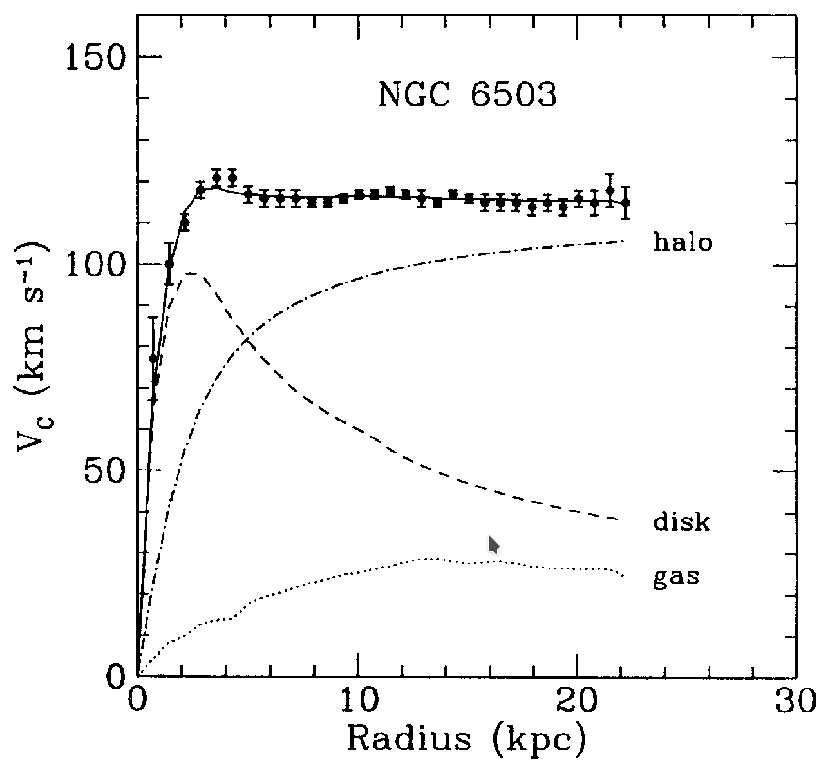
\includegraphics[width=12cm]{F1.png}
\caption{\label{fig:frog} Curva de rotacion galáctica para NGC 6503, vemos el perfil de masa del disco y del gas y el perfil de materia oscura necesario para ajustar los datos.}
\end{figure}
Vamos a describir como se puede utilizar un detector como el CMS en el LHC para hacer busquedas de posibles candidatos a DM, poniendo especial atención en el High Level Trigger (HLT).


\label{sec:examples}

\subsection{CMS en el LHC.}

El Gran Colisionador de Hadrones (LHC) es el acelerador de partículas más grande y energético operado actualmente por la Organización Europea para la Investigación Nuclear (CERN), el LHC usa el mismo tunel de 27 km, cavado en promedio a 100 m de profundidad, del antiguo Gran Colisionador Electrón-Positrón (LEP). EL LHC es capaz de colisionar protones e iones de Plomo con una energía por haz de 7 TeV, sin embargo a día de hoy se hace a 6.5 TeV.
\\

En el LHC están ubicados 4 experimentos principales: LHC-b, ALICE, ATLAS y CMS. Estos últimos dos son detectores de proposito general, es decir, fueron diseñados para detectar señales de nueva física en estados finales de partículas como electrones, fotones, muones y jets de hadrones. El LHC esta dividido en dos partes: la cadena de aceleración y el anillo principal. En la cadena de aceleración los protones son extraídos y pasados por una serie de aceleradores que los llevan hasta una energía de 450 GeV, momento en que son inyectados en el anillo principal. Este está compuesto de dos anillos que llevan los protones en direcciones opuestas,los anillos están construidos por 2090 imanes de 15 m, enfriados a 1.9 K y con un vacío de $10^{-9}$mbar, cada uno capaz de producir un campo magnético de 8,33 T. Además de estos imanes dipolares, el LHC también cuenta con 520 cuadrupolos, 2464 sextupolos y 1232 octupolos usados para colimar el haz. [1]
\\
\\

El Solenoide Compacto de Muones (CMS) es, en tamaño, el segundo experimento más grande del LHC despues de ATLAS, debe su nombre (solenoide compacto) a que varios de los sistemas de detección se encuentran dentro del su gran imán superconductor, capaz de producir un campo magnético uniforme en su interior de 3.8 T y (de muones) debido a que posee un sistema de detección de muones muy preciso y eficiente. CMS es un detector con forma cilíndrica, mide aproximadamente 30 m de largo por 15 m de diámetro, pesa 14000 Ton (esto lo convierte en el experimento más pesado del LHC) y la colaboración se compone de aproximadamente 3500 personas de 182 institutos de física en 41 países. Una representación tres dimensional del detector se puede ver en la figura 2.
\\
\\
\begin{figure}
\centering
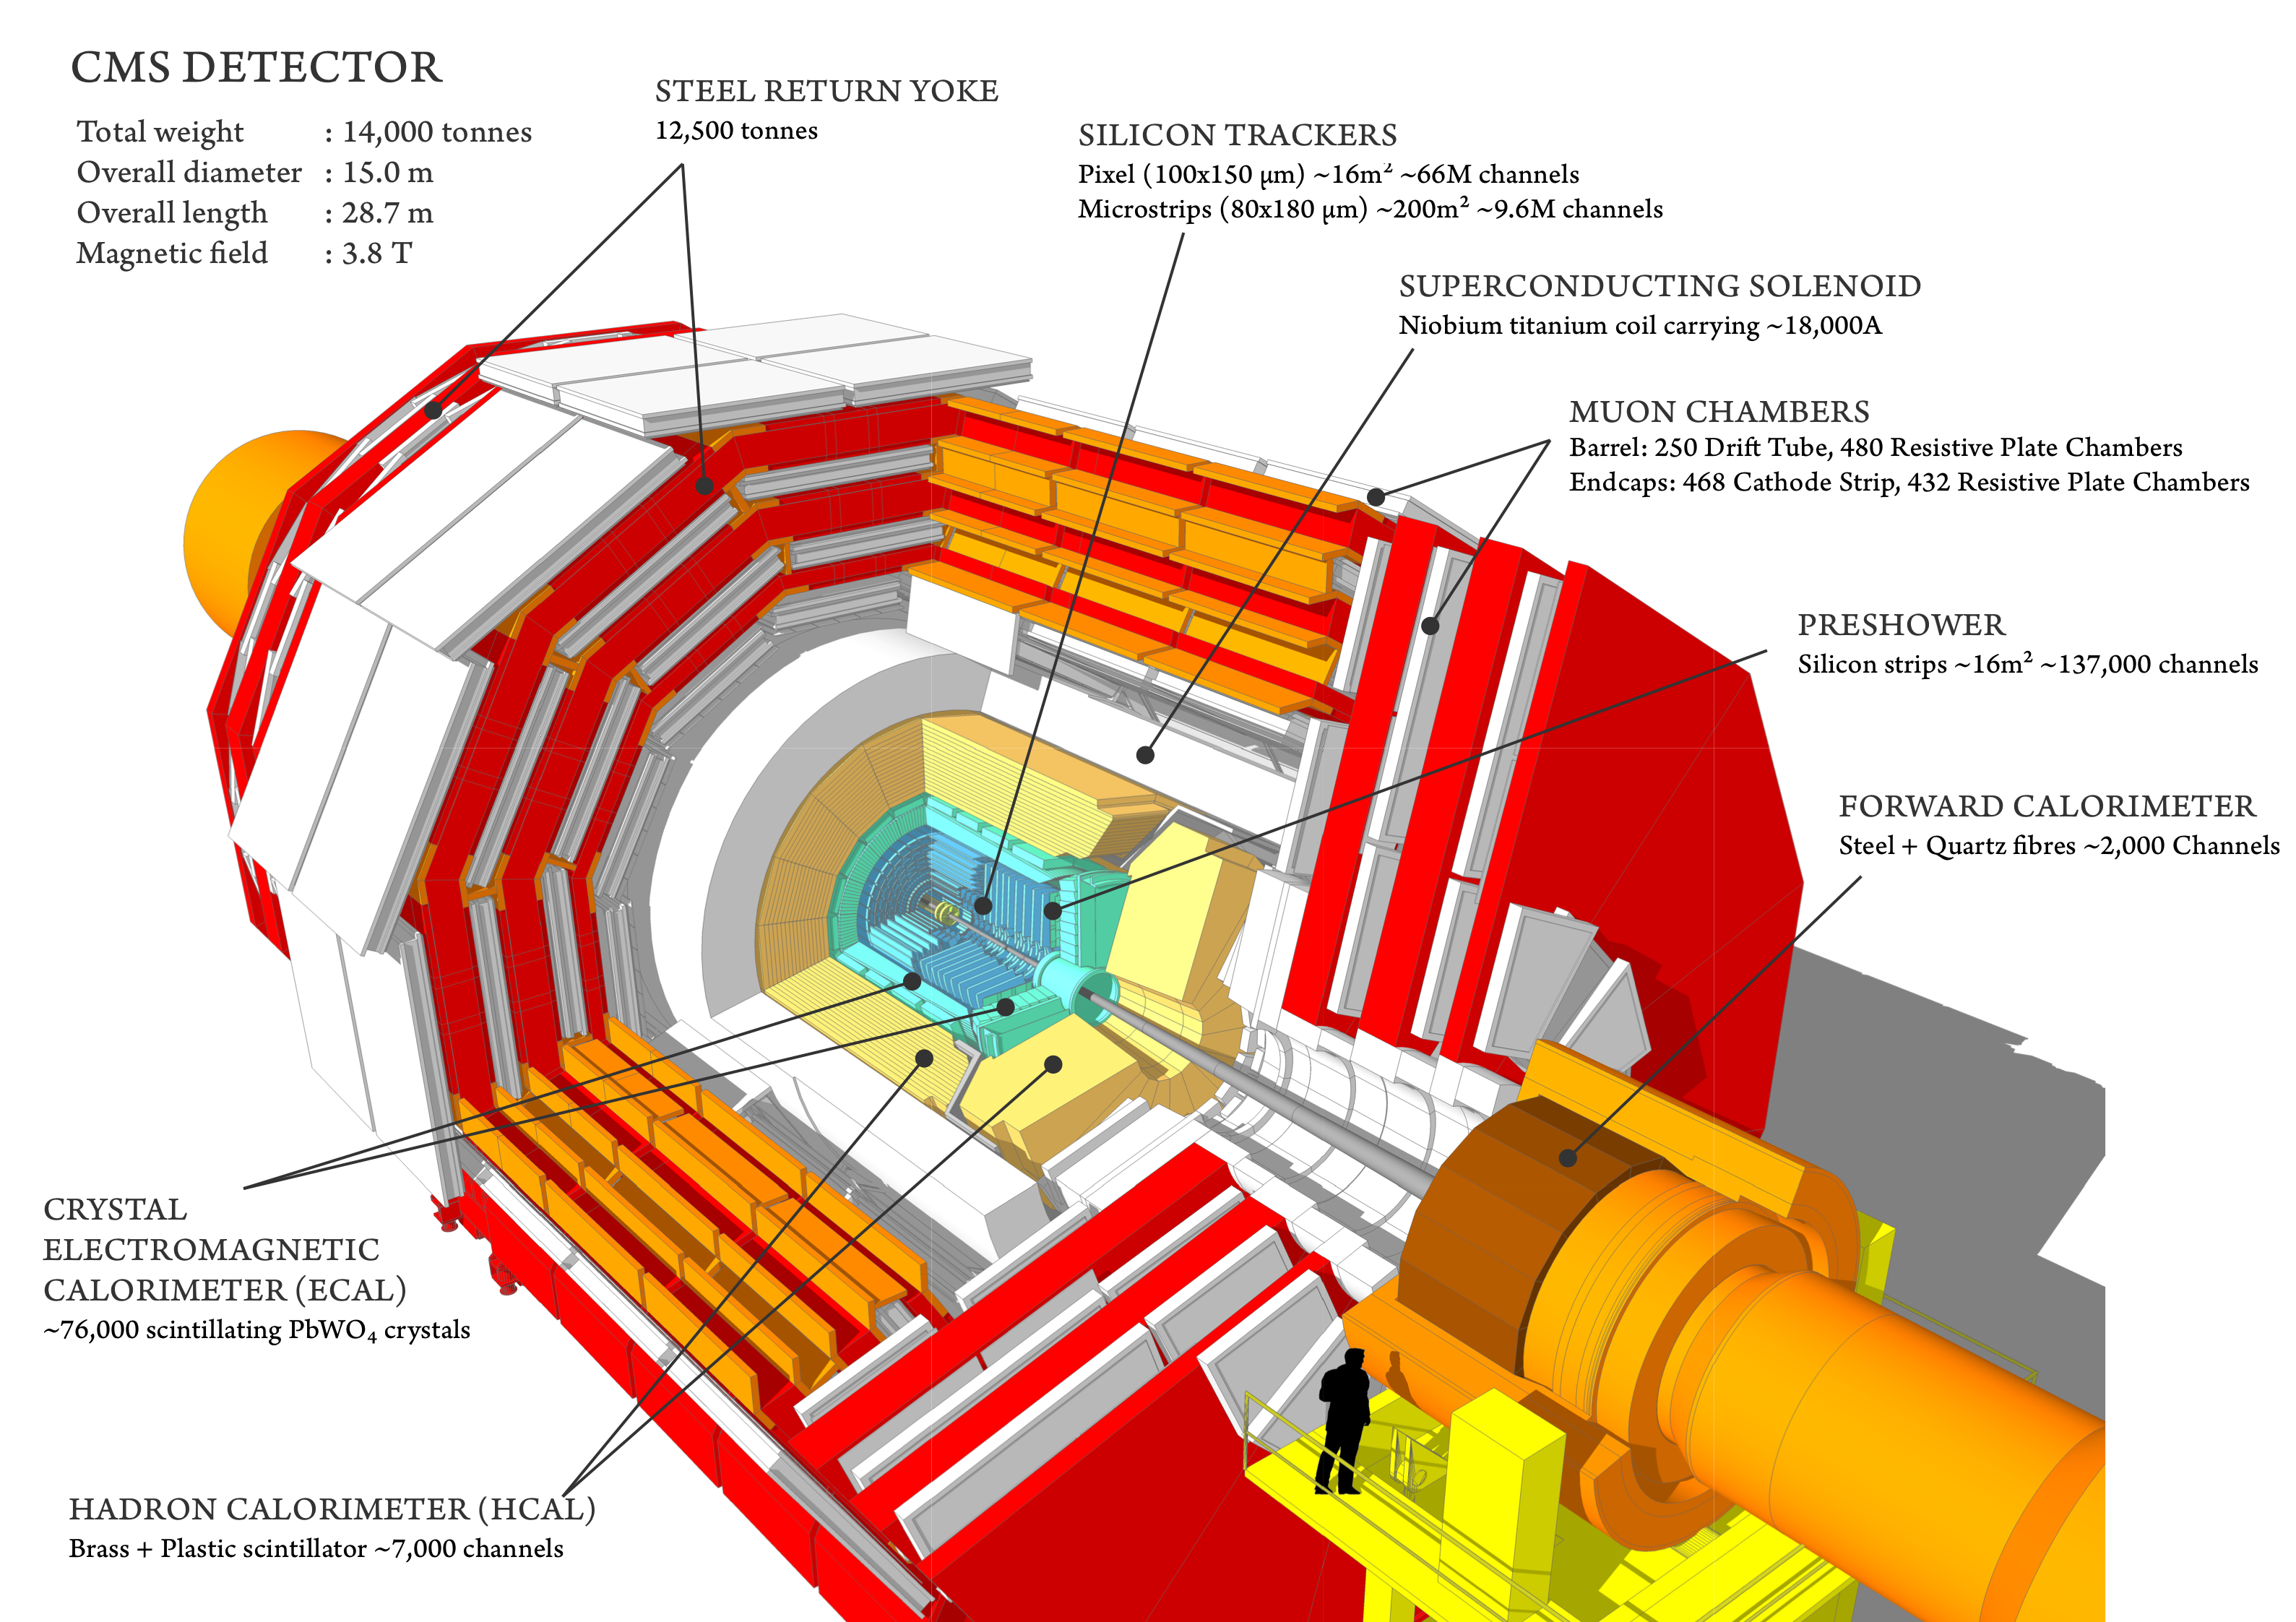
\includegraphics[width=15cm]{F2.png}
\caption{\label{fig:frog} Diseño interno del detector CMS.}
\end{figure}


El imán del CMS tiene 13 m de largo y 6 m de diametro, es capaz de generar un campo magnético uniforme de 4 T en su interior y está construido por 4 capas de espiras de NbTi a 4.45K para que se alcance el estado superconductor, este imán está rodeado por 5 barriles y 3 discos de hierro que tienen el objetivo de devolver el campo magnético generando un campo exterior de 2 T,  esta configuración de campos magnéticos es responsable de curvar las trayectorias de las partículas cargadas.
\\
\\

Dentro del solenoide se encuentra el Tracker System, un sistema de detección diseñado con dos tecnologías: Pixeles y tiras de silicio, está diseñado para identificar los vertices de las colisiones con una precisión de 9 $\mu$m y una eficiencia del 98\% (que se degrada con la luminosidad integrada), cuando una partícula cargada pasa se crean pares electrón-hueco en el material y esto genera una señal eléctrica que luego es amplificada, este sistema fue construido para ser bastante resistente a la radiación y se espera que dure 10 años.
\\
\\
Luego de este sistema se encuentra el calorímetro electromagnético (ECAL), este fue construido para detener electrones y fotones y medir su energía, el sistema está compuesto por cristales de tungstato de plomo, el cual fue escogido por su corta profundidad de radiación, alta densidad y rápido centelleo (25 ns), la unica desventaja del mismo es su alta sensibilidad de respuesta a la temperatura (2\%/C). Los cristales van perdiendo transparencia con la luminosidad integrada y por tanto esta tiene que ser corregida constantemente por un sistema de láser. El sistema cuenta con 61200 cristales en el barril y 7324 en las tapas del calorímetro.
\\
\\
Para detener y detectar los jets hadrónicos se diseñó el calorímetro hadrónico (HCAL), de este sistema cierta parte se encuentra dentro del solenoide (Hadron Endcap Calorimeter y Hadron Barrel Calorimeter) y fuera están el Outer Calorimeter y el Hadron Forward Calorimeter (estos permiten extender el rango angular de detección), los calorímetros tienen el objetivo de detectar los hadrones y lo hacen de la siguiente manera: el sistema tiene intercalados placas de acero con cristales centelladores, las placas de acero generan las duchas de hadrones y cuando estos pasan por los centelladores, la luz generada es convertida en corrientes eléctricas por fotodiodos híbridos (HPDs), estas corrientes permiten medir la energía de los hadrones. Es importante mencionar que debido a la posición del Forward Calorimeter, este recibe mucha radiación comparado a los otros calorìmetros hadrónicos y esto es debido a que está en la dirección del haz incidente y por tanto, los centelladores fueron construidos de un material centellador más resistente a la radiación como lo es el cuarzo.
\\
\\
Finalmente en la parte más externa del detector están ubicados los detectores de muones, esto se debe a que estas partículas tienen un gran poder de penetración. Las cámaras de deteccion están hechas de 3 tecnologías diferentes: Drift Tube Chambers (DT), Cathode Strip Chambers(CSC) y Resistive Plate Chambers (RPC), sin embargo las 3 están basadas en la ionización de gases: al paso de partículas cargadas se generan corrientes de deriva. En la figura 3 se muestra una recreación a un corte transversal del detector.

\begin{figure}
\centering
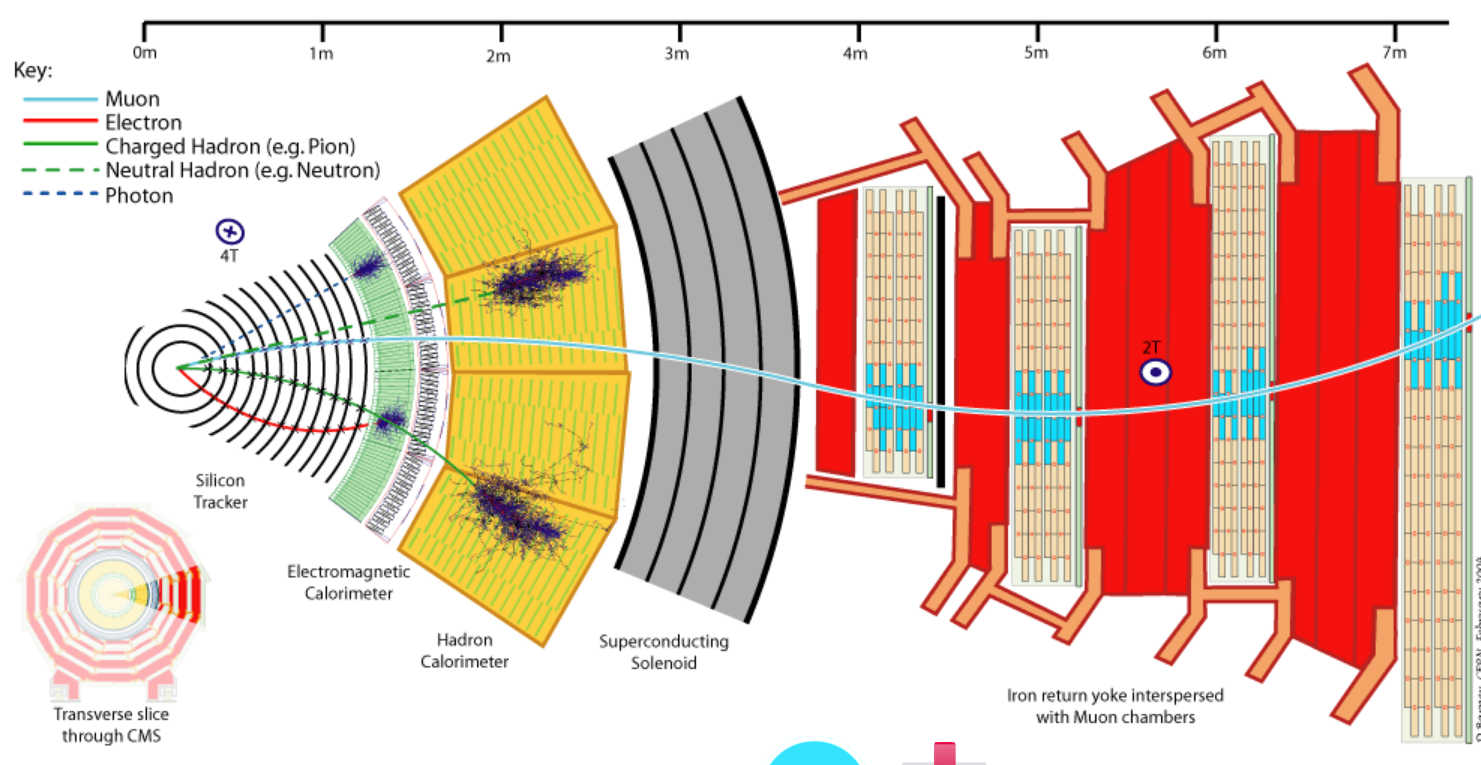
\includegraphics[width=15cm]{F3.png}
\caption{\label{fig:frog} Corte transversal del detector CMS.}
\end{figure}

\subsection{Sistema de Trigger.}

El LHC fue diseñado para tomar los datos de cada colisión que ocurre, cada una está separada en el tiempo por 25 ns, esto produce un flujo de datos de 1 PB/s (PB=Petabyte). Por tanto debe hacerse una selección de eventos en tiempo real, el sistema encargado de hacer esto recibe el nombre de Trigger System y lleva a cabo esta tarea en 2 fases. [2]
\\
\\
La primera de ellas es el Level 1 Trigger (L1), este es un proceso basado en Hardware construido especificamente para analizar los datos provenientes de los sistemas de detección y escoger los eventos más interesantes: aquellos que contienen partículas con gran momento transverso o por ejemplo con combinaciones raras de estados finales. Este filtro reduce el flujo de datos en 2 ordenes de magnitud y dispone de 3.2 $\mu$s para decidir, esto hace que la memoria de almacenamiento deba ser suficiente para guardar los datos de 128  colisiones.
\\
\\
La segunda fase de la selección se conoce como High Level Trigger (HLT) y es un proceso basado en software, una serie de algoritmos corren en granjas de varios miles de procesadores, los códigos han sido previamente implementados con el objetivo de realizar búsquedas predeterminadas y analizan los datos que salen de L1, el tiempo de decisión de este sistema es de aproximadamente 100 ms, al finalizar la selección el flujo original de datos ha sido reducido por un factor de 5 ordenes de magnitud.

\subsection{Materia oscura en colisionadores.}

El modelo estándar de la cosmología predice que solo conocemos como se comporta el 5\% del contenido de materia del universo (materia bariónica), el restante 95\% es: materia oscura (26\%) y energía oscura (69\%) [3], las evidencias de la existencia de materia oscura son variadas y contundentes: lentes gravitacionales, el cúmulo bala, la radiación cósmica de fondo y la estababilidad del gas caliente en clusters de galaxias son algunas de ellas. [4] 
\\
\\
Hace 20 años algunas propuestas a candidatos de materia oscura incluían los MACHOS (Massive compact halo objects), que consisten de objetos astrofísicos muy tenues para ser detectados, por ejemplo: agujeros negros, estrellas de neutrones, enanas blancas, etc. Sin embargo experimentos recientes descartan esta posibilidad y por tanto nos dejan solo con los candidatos no bariónicos como posibles explicaciones. [5,6]
\\
\\
Los candidatos más populares actualmente son los WIMPS (weakly interacting massive particles) y los Axiones, ambas son partículas que surgen como propuesta a la solución de otros problemas en física de partículas (SUSY y CP Fuerte respectivamente) y por esto son tan populares, se sabe que la materia oscura no puede ser caliente, es decir, tener velocidades relativistas, debido a que esto implicaría que el universo fuera más homogéneo de lo que es y tampoco puede interactuar eléctricamente. Otros candidatos para materia oscura surgen de modelos más sencillos como el modelo del doblete inerte y pueden ser detectados en aceleradores como muestran recientes trabajos. [7,8] Esta busqueda en particular se basa en la fusión de bosones vectoriales (VBF) ya que el candidato a materia oscura $H^0$ tiene carga débil. En la figura 4 podemos ver los procesos que contribuyen en este tipo de busquedas, como vemos de los estados finales en los diagramas (jets que se detectan y el candidato de materia oscura escapa), las busquedas se basan en energía transversa faltante (MET) asociada a procesos con dos jets con energía transversa $E_T$ alta y detectados en hemisferios diferentes.
\begin{figure}
	\centering
	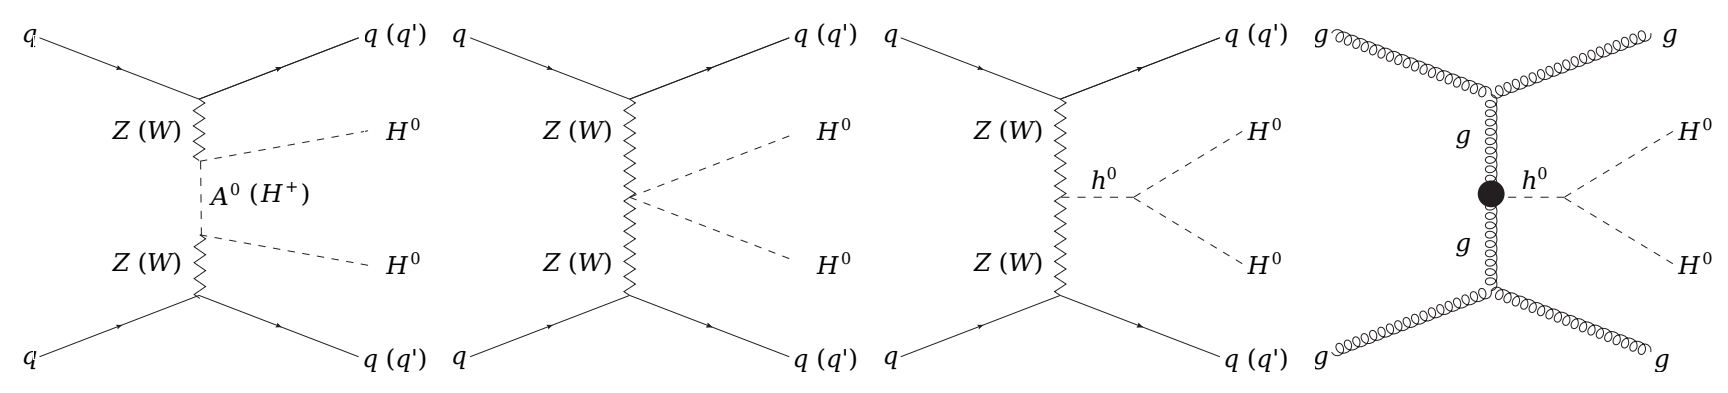
\includegraphics[width=15cm]{F4.png}
	\caption{\label{fig:frog} Diagramas de Feynman que contribuyen a pp$\rightarrow H^0H^0 jj$. El punto en la cuarta figura denota el acople entre el Higgs del modelo estándar y los gluones.}
\end{figure}
\\
\\
Las busquedas en aceleradores como el LHC se basan en la busqueda de estados finales de partículas del modelo estándar con energía transversa faltante [7], de esta manera sabríamos que la partícula de materia oscura vivió lo suficiente como para escapar del detector sin decaer, sin embargo esto no dejaría claro que tan estable es la misma para ser materia oscura y por tanto es necesario complementar la información con experimentos astrofísicos. [9]
\newpage
\section{Problema y pregunta de investigación.}

	Conforme a lo establecido en las secciones anteriores, podemos ver que el problema de encontrar la materia oscura debe resolverse, en parte, mediante la busqueda de la misma en colisionadores, ya hemos visto que modelos como [7,8] motivan busquedas en experimentos como LHC, sin embargo, debido a la cantidad de datos que toman detectores como CMS se deben idear filtros que nos dejen con la información que consideramos relevante a la hora de realizar las busquedas, por tanto nuestra idea es responder: \textbf{¿Qué Hight Level Trigger para el experimento CMS del CERN es pertinente para su uso en el estudio de señales de materia oscura en el detector?}


\newpage
\section{Objetivos y cronograma.}


\subsection{Objetivo general.}

Desarrollar un Hight Level Trigger (HLT) para el experimento CMS del CERN pertinente para su uso en el estudio de señales de materia oscura en el detector.

\subsection{Objetivos específicos.}

\begin{itemize}
	\item Revisión constante de bibliografía.
	\item Estudiar la herramienta de construcción de HLT de CMS.
	\item Estudio del modelo que desea ponerse a prueba, estudianto la señal que quiere detectarse y sus background.
	\item Construcción del HLT usando la herramienta de CMS.
	\item Estudiar la eficiencia y otras características de dicho HLT y proponerlo.
	\item Aplicar el HLT al menos a un modelo específico, un ejemplo podrían ser los modelos [7,8].
\end{itemize}


\subsection{Cronograma.}

\begin{table}[h]
	\centering
	
	\label{my-label}
	\begin{tabular}{|c|c|c|c|c|c|c|c|c|}
		\hline
		Trimestre                              & 2017-3 & 2017-4 & 2018-1 & 2018-2 & 2018-3 & 2018-4 & 2019-1 & 2019-2 \\ \hline
		Revisión de bibliografía.              & *      & *      & *      & *      & *      & *      & *      &        \\ \hline
		Estudio herramienta HLT de CMS.        &        & *      & *      & *      &        &        &        &        \\ \hline
		Estudio fenomenológico.                &        &        & *      & *      &        &        &        &        \\ \hline
		Construcción del HLT                   &        &        &        & *      & *      & *      &        &        \\ \hline
		Estudio de eficiencia.                 &        &        &        &        & *      & *      &        &        \\ \hline
		Aplicar el HLT a un modelo específico. &        &        &        &        &        & *      & *      &        \\ \hline
		Redacción tesis.                       &        &        &        &        &        &        & *      & *      \\ \hline
	\end{tabular}
\end{table}
\section{Infraestructura y recursos.}

\section{Bibliografía.}

[1] Search for a vector-like quark T decaying into top+Higgs in single production mode in full hadronic final state using CMS data collected at 8 TeV, José David Ruiz.
\vspace{0.5cm}

[2] The CMS trigger system, CMS collaboration.

\vspace{0.5cm}

[3] Planck Collaboration, P. A. R. Ade et al., Planck 2015 results. XIII. Cosmo-
logical parameters, arXiv:1502.01589, Astron. Astrophys. 594, A13 (2016).

\vspace{0.5cm}

[4] Status of dark matter in the universe, Katherine Freese.

\vspace{0.5cm}

[5] LIMITS ON STELLAR OBJECTS AS THE DARK MATTER OF OUR HALO: NONBARYONICDARK MATTER SEEMS TO BE REQUIRED, Katherine Freese et al.

\vspace{0.5cm}

[6] SChemical Abundance Constraints on White Dwarfs as Halo Dark Matter, Brian D. Fields et al.

\vspace{0.5cm}

[7] Vector Boson Fusion in the Inert Doublet Model, Bhaskar Dutta, Guillermo Palacio, Diego Restrepo, José D. Ruiz.

\vspace{0.5cm}

[8] Andres G. Delannoy et al., “Probing Dark Matter at the LHC using Vector Boson Fusion
Processes,” Phys. Rev. Lett. 111, 061801 (2013).

\vspace{0.5cm}

[9] Review of Dark Matter searches at colliders, Sarah Alam Malik.


\end{document} to your LaTeX file where you want your

% title page.
%
%%%%%%%%%%%%%%%%%%%%%%%%%%%%%%%%%%%%%%%%%
%\title{Title page with logo}
%----------------------------------------------------------------------------------------
%	PACKAGES AND OTHER DOCUMENT CONFIGURATIONS
%----------------------------------------------------------------------------------------

\documentclass[12pt]{article}
\usepackage[spanish]{babel}
\usepackage[utf8x]{inputenc}
\usepackage{amsmath}
\usepackage{graphicx}
\usepackage[colorinlistoftodos]{todonotes}

\begin{document}

\begin{titlepage}

\newcommand{\HRule}{\rule{\linewidth}{0.5mm}} % Defines a new command for the horizontal lines, change thickness here

\center % Center everything on the page
 
%----------------------------------------------------------------------------------------
%	HEADING SECTIONS
%----------------------------------------------------------------------------------------

\textsc{\LARGE Universidad de Antioquia}\\[1.5cm] % Name of your university/college
\textsc{\Large Facultad de Ciencias Exactas y Naturales}\\[0.5cm]
% Major heading such as course name
\textsc{\Large Instituto de Física}\\[0.5cm]
\textsc{\large Proyecto de Maestría}\\[0.5cm] % Minor heading such as course title

%----------------------------------------------------------------------------------------
%	TITLE SECTION
%----------------------------------------------------------------------------------------

\HRule \\[0.4cm]
{ \huge \bfseries High Level Trigger studies for the detection of dark matter in models with vector like fermions using the CMS detector in the LHC}\\[0.4cm] % Title of your document
\HRule \\[1.5cm]
 
%----------------------------------------------------------------------------------------
%	AUTHOR SECTION
%----------------------------------------------------------------------------------------

\begin{minipage}{0.4\textwidth}
\begin{flushleft} \large
\emph{Autor:}\\
Diego Barón \textsc{} % Your name
\end{flushleft}
\end{minipage}
~
\begin{minipage}{0.4\textwidth}
\begin{flushright} \large
\emph{Asesor:} \\
Nelson Vanegas \textsc{} % Supervisor's Name
\end{flushright}
\end{minipage}\\[1.2cm]

% If you don't want a supervisor, uncomment the two lines below and remove the section above
%\Large \emph{Author:}\\
%John \textsc{Smith}\\[3cm] % Your name

%----------------------------------------------------------------------------------------
%	DATE SECTION
%----------------------------------------------------------------------------------------

{\large \today}\\[0.7cm] % Date, change the \today to a set date if you want to be precise

%----------------------------------------------------------------------------------------
%	LOGO SECTION
%----------------------------------------------------------------------------------------


\includegraphics[width=2.8cm]{udea_fcen.jpg}\\[4cm] % Include a department/university logo - this will requireu the graphicx packag0.7
 
%----------------------------------------------------------------------------------------

\vfill % Fill the rest of the page with whitespace

\end{titlepage}

\tableofcontents % indice de contenidos

\cleardoublepage





\section{Generalidades del proyecto.}

\textbf{Titulo del proyecto:}\\
High Level Trigger studies for the detection of dark matter in models with vector like fermions using the CMS detector in the LHC
\\

\textbf{Línea de investigación:}\\
Física de partículas experimental.
\\

\textbf{Duración:}\\
Dos años.
\\

\textbf{Lugar de ejecución:}\\
Universidad de Antioquia.
\\

\textbf{Equipo de investigación:}\\
\emph{Diego Barón}: Estudiante de maestría.
\emph{Nelson Vanegas}: Asesor, director proyecto UdeA-CMS.
\emph{Jose David Ruíz}: Coasesor, investigador en CMS.
\\

\textbf{Resumen ejecutivo:}\\
En este trabajo se presenta la propuesta de trabajo del estudiante de maestría Diego Barón. Desde 1930 gracias a las observaciones de las curvas de rotacion de las estrellas en las galaxias se plantea la existencia de la materia oscura 


\newpage























\section{Marco conceptual.}
El problema de la materia oscura (DM) es quizás el problema más viejo de la física de partículas, que aún no ha sido satisfactoriamente resuelto, desde 1930 gracias a las observaciones independientes de Lundmark y Zwicky se sabe que el contenido de materia de las galaxias debe ser mayor al que aporta la materia bariónica, en sus experimentos esto se expresaba como el hecho de que las velocidades orbitales del gas y de las estrellas mantiene una tendencia constante respecto a la distancia al centro de la galaxia, en contraposción con lo esperado: que la velocidad decrezca como una función de la distancia. Esto se puede ver en la figura 1.
\\
\\
\begin{figure}
\centering
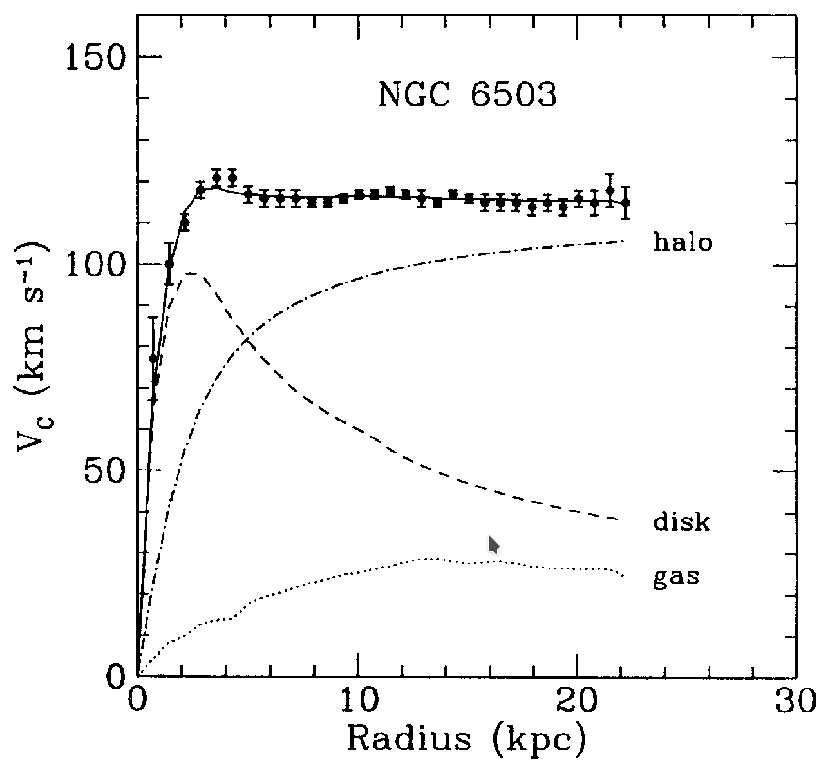
\includegraphics[width=12cm]{F1.png}
\caption{\label{fig:frog} Curva de rotacion galáctica para NGC 6503, vemos el perfil de masa del disco y del gas y el perfil de materia oscura necesario para ajustar los datos.}
\end{figure}
Vamos a describir como se puede utilizar un detector como el CMS en el LHC para hacer busquedas de posibles candidatos a DM, poniendo especial atención en el High Level Trigger (HLT).


\label{sec:examples}

\subsection{CMS en el LHC.}

El Gran Colisionador de Hadrones (LHC) es el acelerador de partículas más grande y energético operado actualmente por la Organización Europea para la Investigación Nuclear (CERN), el LHC usa el mismo tunel de 27 km, cavado en promedio a 100 m de profundidad, del antiguo Gran Colisionador Electrón-Positrón (LEP). EL LHC es capaz de colisionar protones e iones de Plomo con una energía por haz de 7 TeV, sin embargo a día de hoy se hace a 6.5 TeV.
\\

En el LHC están ubicados 4 experimentos principales: LHC-b, ALICE, ATLAS y CMS. Estos últimos dos son detectores de proposito general, es decir, fueron diseñados para detectar señales de nueva física en estados finales de partículas como electrones, fotones, muones y jets de hadrones. El LHC esta dividido en dos partes: la cadena de aceleración y el anillo principal. En la cadena de aceleración los protones son extraídos y pasados por una serie de aceleradores que los llevan hasta una energía de 450 GeV, momento en que son inyectados en el anillo principal. Este está compuesto de dos anillos que llevan los protones en direcciones opuestas,los anillos están construidos por 2090 imanes de 15 m, enfriados a 1.9 K y con un vacío de $10^{-9}$mbar, cada uno capaz de producir un campo magnético de 8,33 T. Además de estos imanes dipolares, el LHC también cuenta con 520 cuadrupolos, 2464 sextupolos y 1232 octupolos usados para colimar el haz. [1]
\\
\\

El Solenoide Compacto de Muones (CMS) es, en tamaño, el segundo experimento más grande del LHC despues de ATLAS, debe su nombre (solenoide compacto) a que varios de los sistemas de detección se encuentran dentro del su gran imán superconductor, capaz de producir un campo magnético uniforme en su interior de 3.8 T y (de muones) debido a que posee un sistema de detección de muones muy preciso y eficiente. CMS es un detector con forma cilíndrica, mide aproximadamente 30 m de largo por 15 m de diámetro, pesa 14000 Ton (esto lo convierte en el experimento más pesado del LHC) y la colaboración se compone de aproximadamente 3500 personas de 182 institutos de física en 41 países. Una representación tres dimensional del detector se puede ver en la figura 2.
\\
\\
\begin{figure}
\centering
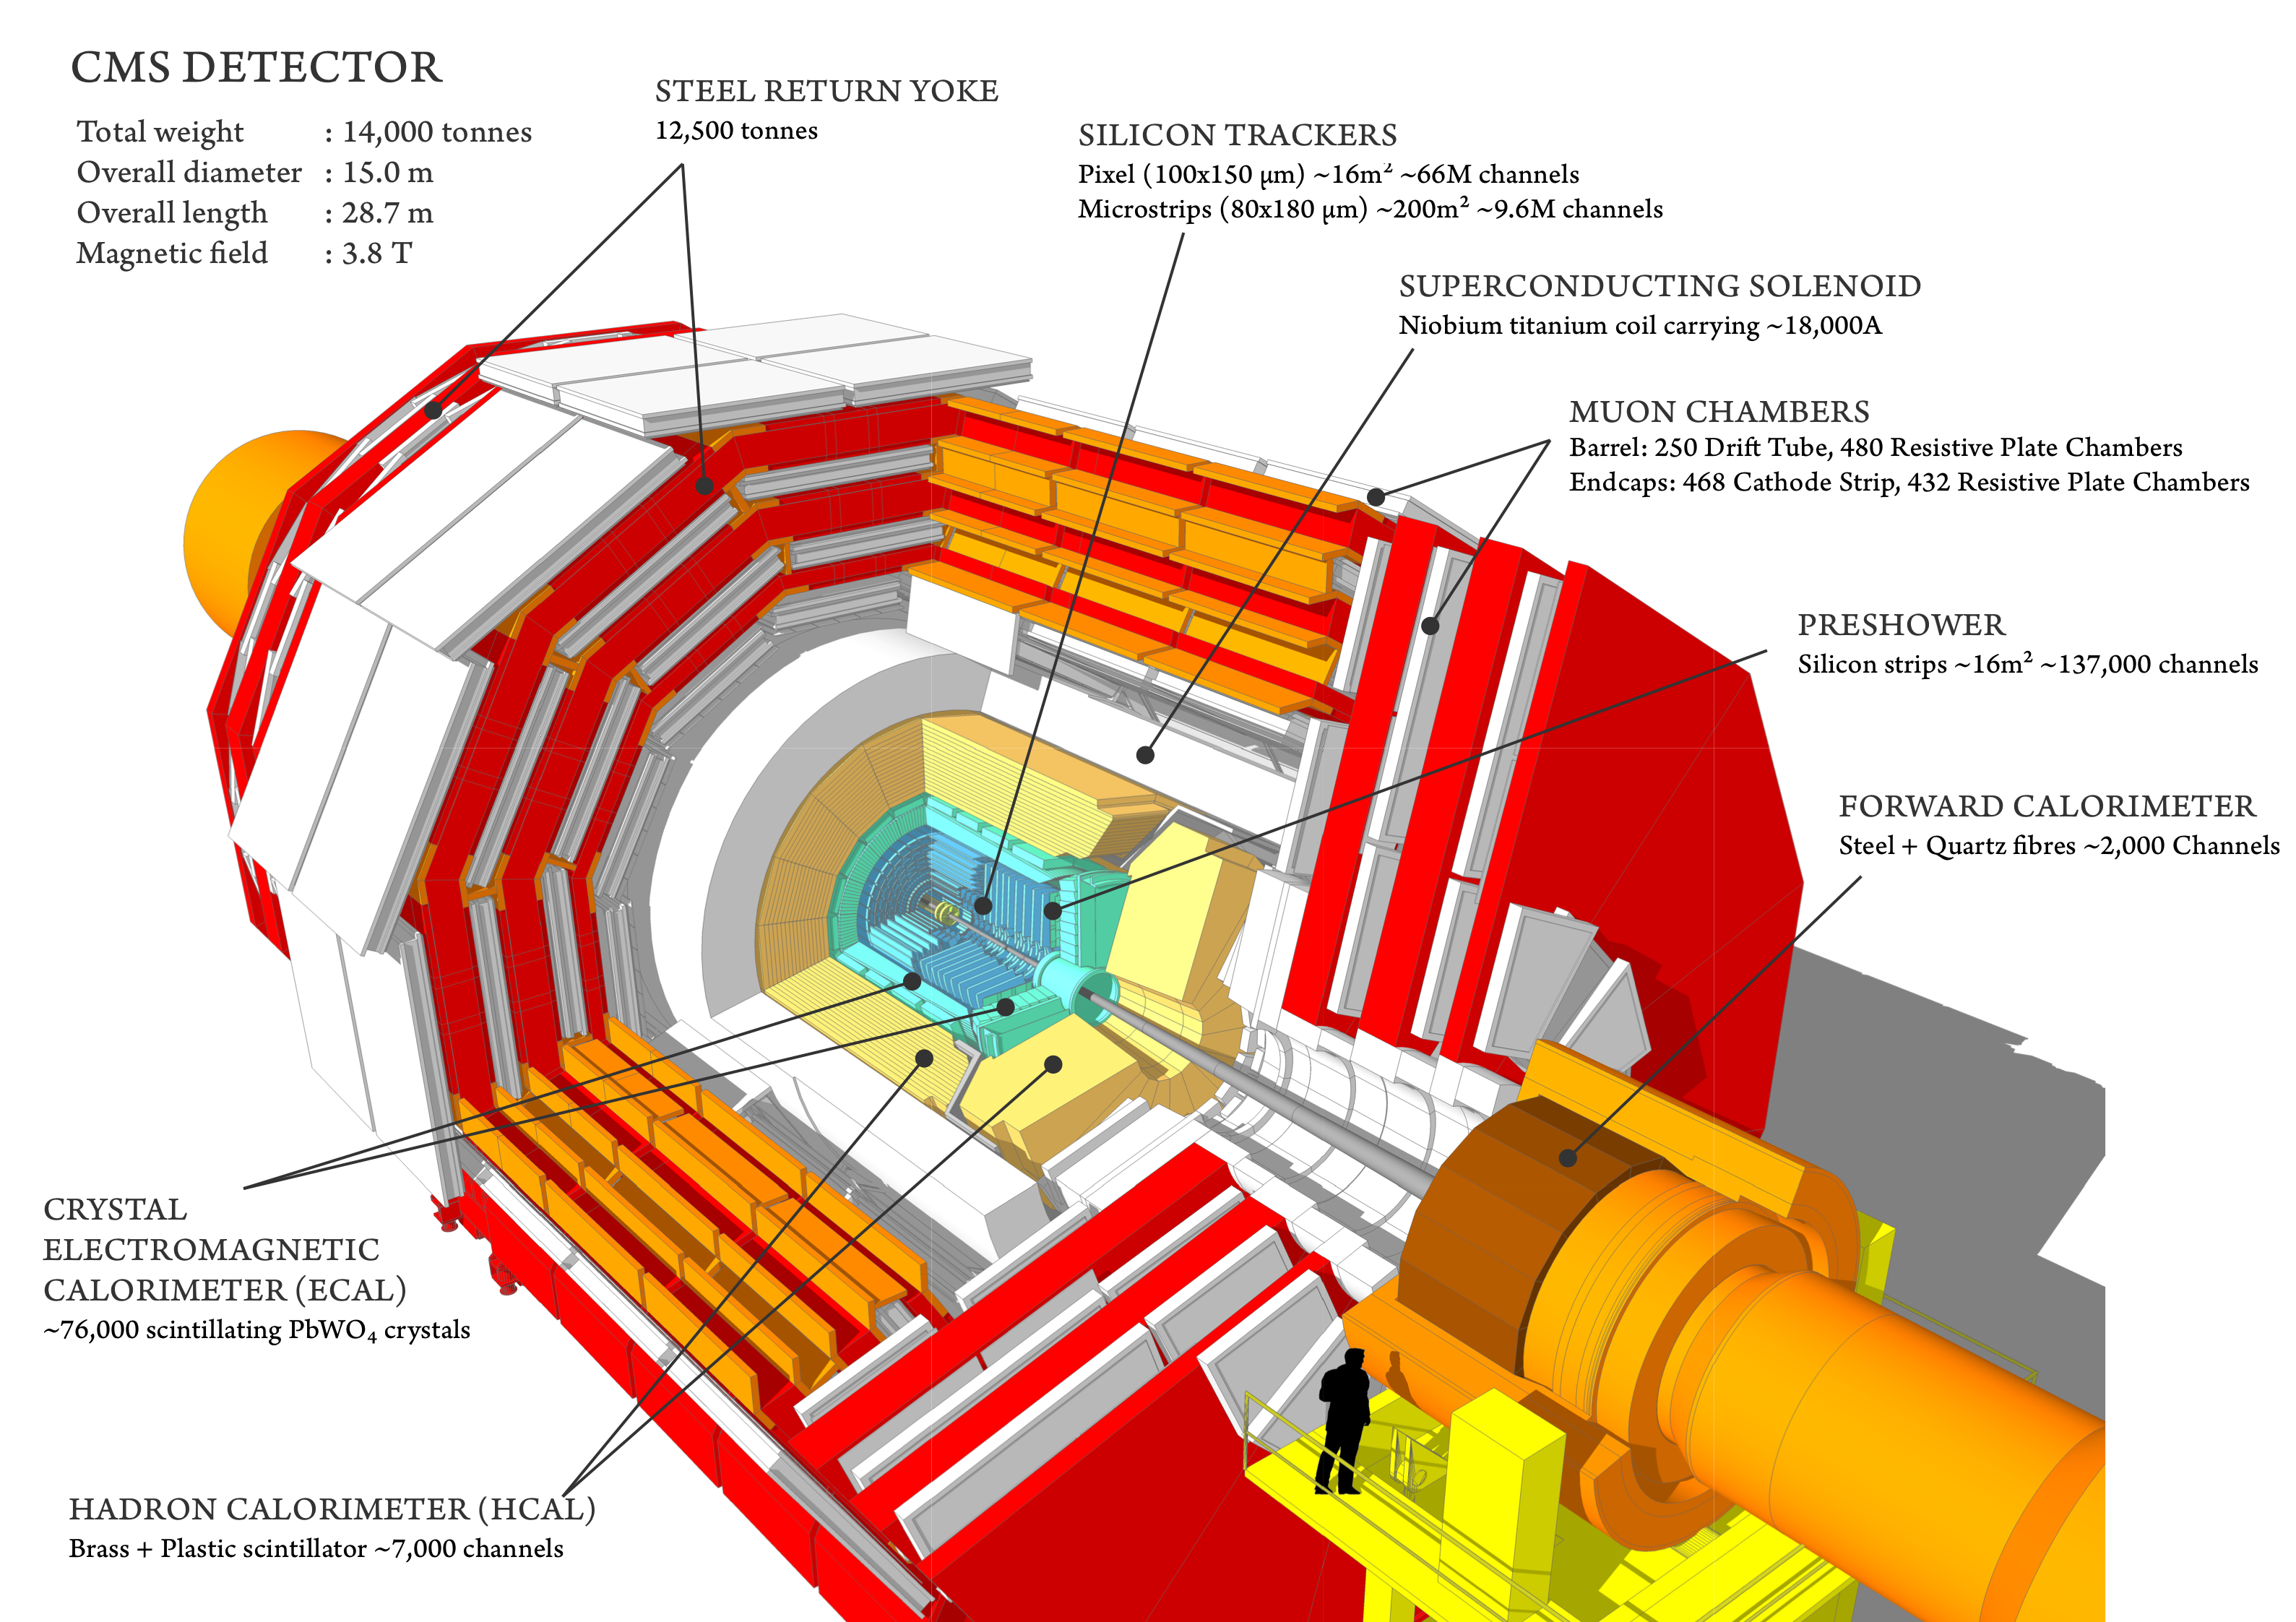
\includegraphics[width=15cm]{F2.png}
\caption{\label{fig:frog} Diseño interno del detector CMS.}
\end{figure}


El imán del CMS tiene 13 m de largo y 6 m de diametro, es capaz de generar un campo magnético uniforme de 4 T en su interior y está construido por 4 capas de espiras de NbTi a 4.45K para que se alcance el estado superconductor, este imán está rodeado por 5 barriles y 3 discos de hierro que tienen el objetivo de devolver el campo magnético generando un campo exterior de 2 T,  esta configuración de campos magnéticos es responsable de curvar las trayectorias de las partículas cargadas.
\\
\\

Dentro del solenoide se encuentra el Tracker System, un sistema de detección diseñado con dos tecnologías: Pixeles y tiras de silicio, está diseñado para identificar los vertices de las colisiones con una precisión de 9 $\mu$m y una eficiencia del 98\% (que se degrada con la luminosidad integrada), cuando una partícula cargada pasa se crean pares electrón-hueco en el material y esto genera una señal eléctrica que luego es amplificada, este sistema fue construido para ser bastante resistente a la radiación y se espera que dure 10 años.
\\
\\
Luego de este sistema se encuentra el calorímetro electromagnético (ECAL), este fue construido para detener electrones y fotones y medir su energía, el sistema está compuesto por cristales de tungstato de plomo, el cual fue escogido por su corta profundidad de radiación, alta densidad y rápido centelleo (25 ns), la unica desventaja del mismo es su alta sensibilidad de respuesta a la temperatura (2\%/C). Los cristales van perdiendo transparencia con la luminosidad integrada y por tanto esta tiene que ser corregida constantemente por un sistema de láser. El sistema cuenta con 61200 cristales en el barril y 7324 en las tapas del calorímetro.
\\
\\
Para detener y detectar los jets hadrónicos se diseñó el calorímetro hadrónico (HCAL), de este sistema cierta parte se encuentra dentro del solenoide (Hadron Endcap Calorimeter y Hadron Barrel Calorimeter) y fuera están el Outer Calorimeter y el Hadron Forward Calorimeter (estos permiten extender el rango angular de detección), los calorímetros tienen el objetivo de detectar los hadrones y lo hacen de la siguiente manera: el sistema tiene intercalados placas de acero con cristales centelladores, las placas de acero generan las duchas de hadrones y cuando estos pasan por los centelladores, la luz generada es convertida en corrientes eléctricas por fotodiodos híbridos (HPDs), estas corrientes permiten medir la energía de los hadrones. Es importante mencionar que debido a la posición del Forward Calorimeter, este recibe mucha radiación comparado a los otros calorìmetros hadrónicos y esto es debido a que está en la dirección del haz incidente y por tanto, los centelladores fueron construidos de un material centellador más resistente a la radiación como lo es el cuarzo.
\\
\\
Finalmente en la parte más externa del detector están ubicados los detectores de muones, esto se debe a que estas partículas tienen un gran poder de penetración. Las cámaras de deteccion están hechas de 3 tecnologías diferentes: Drift Tube Chambers (DT), Cathode Strip Chambers(CSC) y Resistive Plate Chambers (RPC), sin embargo las 3 están basadas en la ionización de gases: al paso de partículas cargadas se generan corrientes de deriva. En la figura 3 se muestra una recreación a un corte transversal del detector.

\begin{figure}
\centering
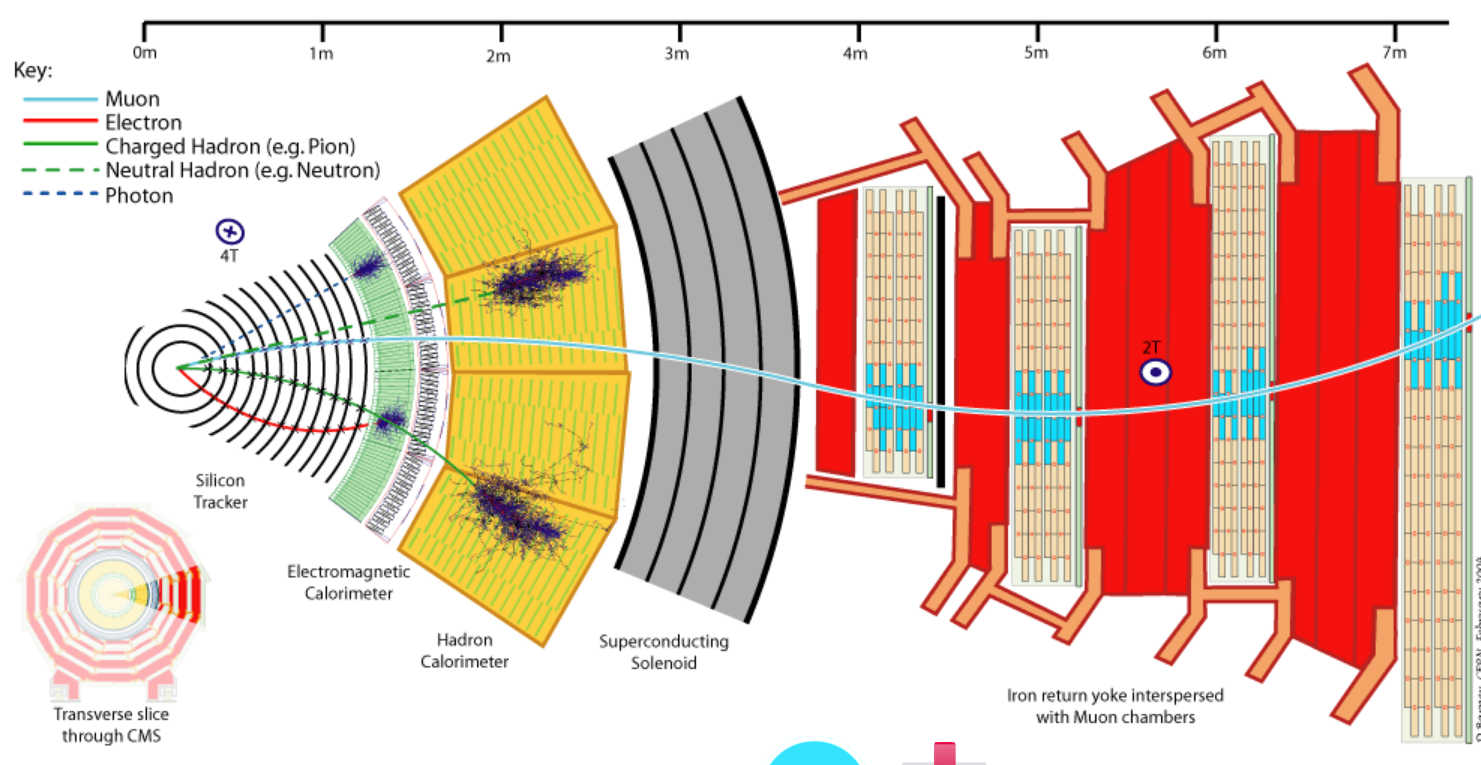
\includegraphics[width=15cm]{F3.png}
\caption{\label{fig:frog} Corte transversal del detector CMS.}
\end{figure}

\subsection{Sistema de Trigger.}

El LHC fue diseñado para tomar los datos de cada colisión que ocurre, cada una está separada en el tiempo por 25 ns, esto produce un flujo de datos de 1 PB/s (PB=Petabyte). Por tanto debe hacerse una selección de eventos en tiempo real, el sistema encargado de hacer esto recibe el nombre de Trigger System y lleva a cabo esta tarea en 2 fases. [2]
\\
\\
La primera de ellas es el Level 1 Trigger (L1), este es un proceso basado en Hardware construido especificamente para analizar los datos provenientes de los sistemas de detección y escoger los eventos más interesantes: aquellos que contienen partículas con gran momento transverso o por ejemplo con combinaciones raras de estados finales. Este filtro reduce el flujo de datos en 2 ordenes de magnitud y dispone de 3.2 $\mu$s para decidir, esto hace que la memoria de almacenamiento deba ser suficiente para guardar los datos de 128  colisiones.
\\
\\
La segunda fase de la selección se conoce como High Level Trigger (HLT) y es un proceso basado en software, una serie de algoritmos corren en granjas de varios miles de procesadores, los códigos han sido previamente implementados con el objetivo de realizar búsquedas predeterminadas y analizan los datos que salen de L1, el tiempo de decisión de este sistema es de aproximadamente 100 ms, al finalizar la selección el flujo original de datos ha sido reducido por un factor de 5 ordenes de magnitud.

\subsection{Materia oscura en colisionadores.}

El modelo estándar de la cosmología predice que solo conocemos como se comporta el 5\% del contenido de materia del universo (materia bariónica), el restante 95\% es: materia oscura (26\%) y energía oscura (69\%) [3], las evidencias de la existencia de materia oscura son variadas y contundentes: lentes gravitacionales, el cúmulo bala, la radiación cósmica de fondo y la estababilidad del gas caliente en clusters de galaxias son algunas de ellas. [4] 
\\
\\
Hace 20 años algunas propuestas a candidatos de materia oscura incluían los MACHOS (Massive compact halo objects), que consisten de objetos astrofísicos muy tenues para ser detectados, por ejemplo: agujeros negros, estrellas de neutrones, enanas blancas, etc. Sin embargo experimentos recientes descartan esta posibilidad y por tanto nos dejan solo con los candidatos no bariónicos como posibles explicaciones. [5,6]
\\
\\
Los candidatos más populares actualmente son los WIMPS (weakly interacting massive particles) y los Axiones, ambas son partículas que surgen como propuesta a la solución de otros problemas en física de partículas (SUSY y CP Fuerte respectivamente) y por esto son tan populares, se sabe que la materia oscura no puede ser caliente, es decir, tener velocidades relativistas, debido a que esto implicaría que el universo fuera más homogéneo de lo que es y tampoco puede interactuar eléctricamente. Otros candidatos para materia oscura surgen de modelos más sencillos como el modelo del doblete inerte y pueden ser detectados en aceleradores como muestran recientes trabajos. [7,8] Esta busqueda en particular se basa en la fusión de bosones vectoriales (VBF) ya que el candidato a materia oscura $H^0$ tiene carga débil. En la figura 4 podemos ver los procesos que contribuyen en este tipo de busquedas, como vemos de los estados finales en los diagramas (jets que se detectan y el candidato de materia oscura escapa), las busquedas se basan en energía transversa faltante (MET) asociada a procesos con dos jets con energía transversa $E_T$ alta y detectados en hemisferios diferentes.
\begin{figure}
	\centering
	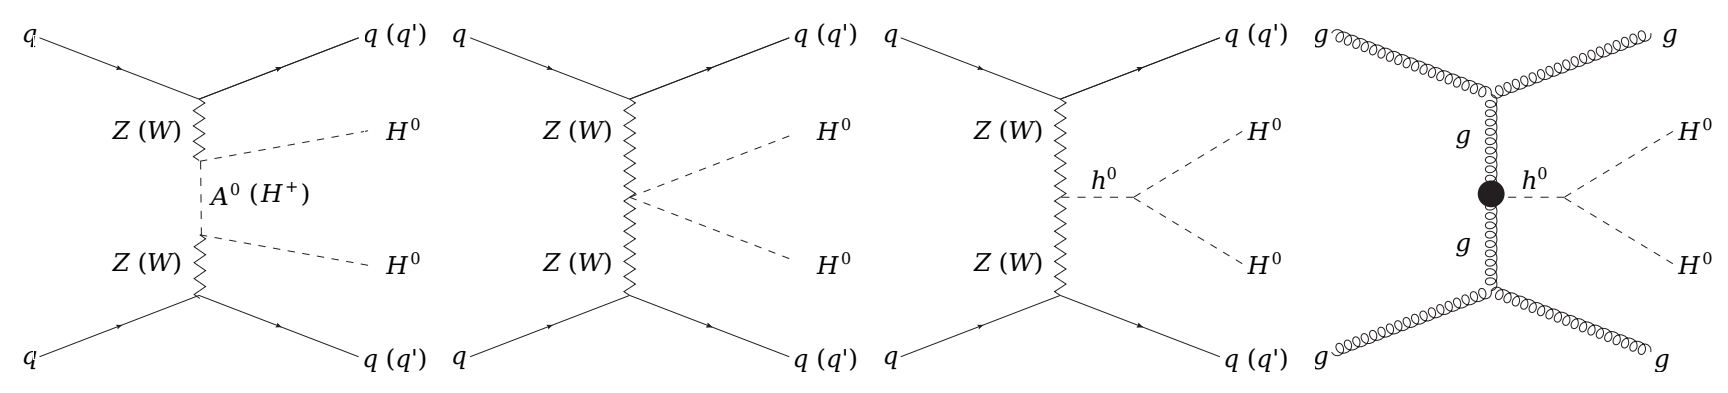
\includegraphics[width=15cm]{F4.png}
	\caption{\label{fig:frog} Diagramas de Feynman que contribuyen a pp$\rightarrow H^0H^0 jj$. El punto en la cuarta figura denota el acople entre el Higgs del modelo estándar y los gluones.}
\end{figure}
\\
\\
Las busquedas en aceleradores como el LHC se basan en la busqueda de estados finales de partículas del modelo estándar con energía transversa faltante [7], de esta manera sabríamos que la partícula de materia oscura vivió lo suficiente como para escapar del detector sin decaer, sin embargo esto no dejaría claro que tan estable es la misma para ser materia oscura y por tanto es necesario complementar la información con experimentos astrofísicos. [9]
\newpage
\section{Problema y pregunta de investigación.}

	Conforme a lo establecido en las secciones anteriores, podemos ver que el problema de encontrar la materia oscura debe resolverse, en parte, mediante la busqueda de la misma en colisionadores, ya hemos visto que modelos como [7,8] motivan busquedas en experimentos como LHC, sin embargo, debido a la cantidad de datos que toman detectores como CMS se deben idear filtros que nos dejen con la información que consideramos relevante a la hora de realizar las busquedas, por tanto nuestra idea es responder: \textbf{¿Qué Hight Level Trigger para el experimento CMS del CERN es pertinente para su uso en el estudio de señales de materia oscura en el detector?}


\newpage
\section{Objetivos y cronograma.}


\subsection{Objetivo general.}

Desarrollar un Hight Level Trigger (HLT) para el experimento CMS del CERN pertinente para su uso en el estudio de señales de materia oscura en el detector.

\subsection{Objetivos específicos.}

\begin{itemize}
	\item Revisión constante de bibliografía.
	\item Estudiar la herramienta de construcción de HLT de CMS.
	\item Estudio del modelo que desea ponerse a prueba, estudianto la señal que quiere detectarse y sus background.
	\item Construcción del HLT usando la herramienta de CMS.
	\item Estudiar la eficiencia y otras características de dicho HLT y proponerlo.
	\item Aplicar el HLT al menos a un modelo específico, un ejemplo podrían ser los modelos [7,8].
\end{itemize}


\subsection{Cronograma.}

\begin{table}[h]
	\centering
	
	\label{my-label}
	\begin{tabular}{|c|c|c|c|c|c|c|c|c|}
		\hline
		Trimestre                              & 2017-3 & 2017-4 & 2018-1 & 2018-2 & 2018-3 & 2018-4 & 2019-1 & 2019-2 \\ \hline
		Revisión de bibliografía.              & *      & *      & *      & *      & *      & *      & *      &        \\ \hline
		Estudio herramienta HLT de CMS.        &        & *      & *      & *      &        &        &        &        \\ \hline
		Estudio fenomenológico.                &        &        & *      & *      &        &        &        &        \\ \hline
		Construcción del HLT                   &        &        &        & *      & *      & *      &        &        \\ \hline
		Estudio de eficiencia.                 &        &        &        &        & *      & *      &        &        \\ \hline
		Aplicar el HLT a un modelo específico. &        &        &        &        &        & *      & *      &        \\ \hline
		Redacción tesis.                       &        &        &        &        &        &        & *      & *      \\ \hline
	\end{tabular}
\end{table}
\section{Infraestructura y recursos.}

\section{Bibliografía.}

[1] Search for a vector-like quark T decaying into top+Higgs in single production mode in full hadronic final state using CMS data collected at 8 TeV, José David Ruiz.
\vspace{0.5cm}

[2] The CMS trigger system, CMS collaboration.

\vspace{0.5cm}

[3] Planck Collaboration, P. A. R. Ade et al., Planck 2015 results. XIII. Cosmo-
logical parameters, arXiv:1502.01589, Astron. Astrophys. 594, A13 (2016).

\vspace{0.5cm}

[4] Status of dark matter in the universe, Katherine Freese.

\vspace{0.5cm}

[5] LIMITS ON STELLAR OBJECTS AS THE DARK MATTER OF OUR HALO: NONBARYONICDARK MATTER SEEMS TO BE REQUIRED, Katherine Freese et al.

\vspace{0.5cm}

[6] SChemical Abundance Constraints on White Dwarfs as Halo Dark Matter, Brian D. Fields et al.

\vspace{0.5cm}

[7] Vector Boson Fusion in the Inert Doublet Model, Bhaskar Dutta, Guillermo Palacio, Diego Restrepo, José D. Ruiz.

\vspace{0.5cm}

[8] Andres G. Delannoy et al., “Probing Dark Matter at the LHC using Vector Boson Fusion
Processes,” Phys. Rev. Lett. 111, 061801 (2013).

\vspace{0.5cm}

[9] Review of Dark Matter searches at colliders, Sarah Alam Malik.


\end{document} to your LaTeX file where you want your

% title page.
%
%%%%%%%%%%%%%%%%%%%%%%%%%%%%%%%%%%%%%%%%%
%\title{Title page with logo}
%----------------------------------------------------------------------------------------
%	PACKAGES AND OTHER DOCUMENT CONFIGURATIONS
%----------------------------------------------------------------------------------------

\documentclass[12pt]{article}
\usepackage[spanish]{babel}
\usepackage[utf8x]{inputenc}
\usepackage{amsmath}
\usepackage{graphicx}
\usepackage[colorinlistoftodos]{todonotes}

\begin{document}

\begin{titlepage}

\newcommand{\HRule}{\rule{\linewidth}{0.5mm}} % Defines a new command for the horizontal lines, change thickness here

\center % Center everything on the page
 
%----------------------------------------------------------------------------------------
%	HEADING SECTIONS
%----------------------------------------------------------------------------------------

\textsc{\LARGE Universidad de Antioquia}\\[1.5cm] % Name of your university/college
\textsc{\Large Facultad de Ciencias Exactas y Naturales}\\[0.5cm]
% Major heading such as course name
\textsc{\Large Instituto de Física}\\[0.5cm]
\textsc{\large Proyecto de Maestría}\\[0.5cm] % Minor heading such as course title

%----------------------------------------------------------------------------------------
%	TITLE SECTION
%----------------------------------------------------------------------------------------

\HRule \\[0.4cm]
{ \huge \bfseries High Level Trigger studies for the detection of dark matter in models with vector like fermions using the CMS detector at the LHC}\\[0.4cm] % Title of your document
\HRule \\[1.5cm]
 
%----------------------------------------------------------------------------------------
%	AUTHOR SECTION
%----------------------------------------------------------------------------------------

\begin{minipage}{0.4\textwidth}
\begin{flushleft} \large
\emph{Autor:}\\
Diego Barón \textsc{} % Your name
\end{flushleft}
\end{minipage}
~
\begin{minipage}{0.4\textwidth}
\begin{flushright} \large
\emph{Asesor:} \\
Nelson Vanegas \textsc{} % Supervisor's Name
\end{flushright}
\end{minipage}\\[1.2cm]

% If you don't want a supervisor, uncomment the two lines below and remove the section above
%\Large \emph{Author:}\\
%John \textsc{Smith}\\[3cm] % Your name

%----------------------------------------------------------------------------------------
%	DATE SECTION
%----------------------------------------------------------------------------------------

{\large \today}\\[0.7cm] % Date, change the \today to a set date if you want to be precise

%----------------------------------------------------------------------------------------
%	LOGO SECTION
%----------------------------------------------------------------------------------------


\includegraphics[width=2.8cm]{udea_fcen.jpg}\\[4cm] % Include a department/university logo - this will requireu the graphicx packag0.7
 
%----------------------------------------------------------------------------------------

\vfill % Fill the rest of the page with whitespace

\end{titlepage}

\tableofcontents % indice de contenidos

\cleardoublepage





\section{Generalidades del proyecto}

\textbf{Título del proyecto:}\\
High Level Trigger studies for the detection of dark matter in models with vector like fermions using the CMS detector at the LHC
\\

\textbf{Línea de investigación:}\\
Física de partículas experimental.
\\

\textbf{Duración:}\\
Dos años.
\\

\textbf{Lugar de ejecución:}\\
Universidad de Antioquia.
\\

\textbf{Equipo de investigación:}\\
\emph{Diego Barón}: Estudiante de maestría.
\emph{Nelson Vanegas}: Asesor, director proyecto UdeA-CMS.
\emph{Jose David Ruíz}: Coasesor, investigador en CMS.
\\

\textbf{Resumen ejecutivo:}\\
En este trabajo se presenta la propuesta de trabajo del estudiante de maestría Diego Alberto Barón Moreno. Desde 1930, gracias a las observaciones de las curvas de rotación de las estrellas en las galaxias, se plantea la existencia de la materia oscura. En un acelerador de partículas como el Gran Colisionador de Hadrones (LHC) se colisionan haces de protones e iones de plomo y en estas colisiones, en principio, se pueden generar las partículas que constituyen la materia oscura en el universo. Sin embargo, debido a la gran cantidad de datos que toman los detectores del LHC, como el Solenoide Compacto de Muones (CMS)\cite{Bayatian:2006nff}, se deben aplicar filtros para aislar los eventos interesantes. En este trabajo proponemos desarrollar un filtro de eventos de alto nivel (en inglés path High Level Trigger), es decir: una serie de algoritmos de selección de eventos, que se ejecutan luego de la obtención de datos en el detector CMS. El objetivo es que este path High Level Trigger (HLT path) sea adecuado para la búsqueda de materia osucura (DM) en el detector CMS en el LHC.


\newpage























\section{Marco conceptual}
El problema de la materia oscura (DM) es el problema más viejo de la física de partículas, que aún no ha sido satisfactoriamente resuelto. Desde 1930 gracias a las observaciones independientes de Lundmark y Zwicky \cite{ARTICLE:1,ARTICLE:2} se sabe que el contenido de materia de las galaxias debe ser mayor al que aporta la materia bariónica. En sus experimentos ellos encontraron que las velocidades orbitales del gas y de las estrellas mantienen una tendencia constante respecto a la distancia al centro de la galaxia.
 Esto está en contraposción con lo que se espera al aplicar las leyes de Newton de la gravitación: que la velocidad decrezca como una función de la distancia. Esto se puede ver en la figura 1.
\\
\\
\begin{figure}
\centering
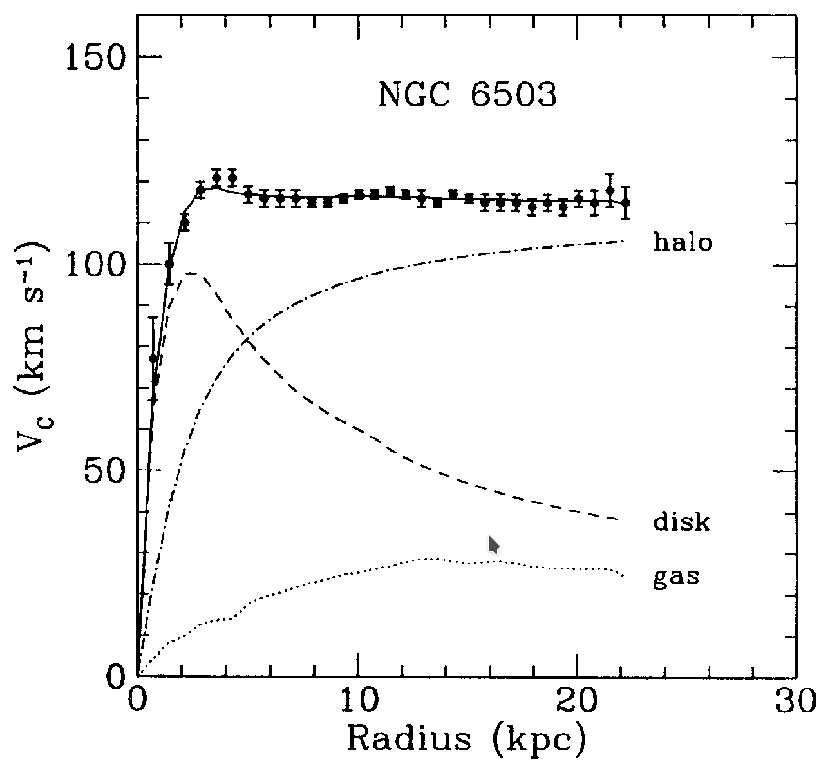
\includegraphics[width=12cm]{F1.png}
\caption{\label{fig:frog} Curva de rotacion galáctica para NGC 6503, vemos el perfil de masa del disco y del gas y el perfil de materia oscura necesario para ajustar los datos. Tomado de \cite{Freese:2017idy}.}
\end{figure}
A continuación vamos a describir los componentes fundamentales del detector CMS en el LHC, poniendo especial atención en el sitema High Level Trigger.


\label{sec:examples}

\subsection{CMS en el LHC}

El Gran Colisionador de Hadrones es el acelerador de partículas más grande y energético operado actualmente por la Organización Europea para la Investigación Nuclear (CERN). El LHC usa el mismo tunel de 27 km, cavado en promedio a 100 m de profundidad, del antiguo Gran Colisionador Electrón-Positrón (LEP). EL LHC es capaz de colisionar protones con una energía por haz de 7 TeV, sin embargo a día de hoy se hace a 6.5 TeV.
\\

En el LHC están ubicados 4 experimentos principales: LHC-b \cite{Alves:2008zz}, ALICE \cite{Aamodt:2008zz}, ATLAS \cite{Aad:2008zzm} y CMS. Estos últimos dos son detectores de proposito general, es decir, fueron diseñados para detectar señales de nueva física en estados finales de partículas como electrones, fotones, muones y jets de hadrones. El LHC esta dividido en dos partes: la cadena de aceleración y el anillo principal. En la cadena de aceleración los protones son extraídos y pasados por una serie de aceleradores que los llevan hasta una energía de 450 GeV, momento en que son inyectados en el anillo principal. El anillo principal está compuesto de dos anillos que llevan los protones en direcciones opuestas, los anillos están construidos por 2090 imanes dipolares y superconductores de 15 m de largo, enfriados a 1.9 K y con un vacío de $10^{-9}$mbar; cada uno capaz de producir un campo magnético de 8,33 T. Además de estos imanes dipolares, el LHC también cuenta con 520 cuadrupolos, 2464 sextupolos y 1232 octupolos usados para colimar el haz \cite{RuizAlvarez:2016mhn}. 
\\
\\

El Solenoide Compacto de Muones (CMS) es en tamaño, el segundo experimento más grande del LHC despues de ATLAS. CMS debe su nombre ``solenoide compacto'' a que varios de los sistemas de detección se encuentran dentro de su gran imán superconductor, capaz de producir un campo magnético uniforme en su interior de 3.8 T. Y ``solenoide de muones'' debido a que posee un sistema de detección de muones muy preciso y eficiente. CMS es un detector con forma cilíndrica, mide aproximadamente 30 m de largo por 15 m de diámetro y pesa 14000 Ton (esto lo convierte en el experimento más pesado del LHC). La colaboración se compone de aproximadamente 3500 personas de 182 institutos de física en 41 países. Una representación tres dimensional del detector se puede ver en la figura 2.
\\
\\
\begin{figure}
\centering
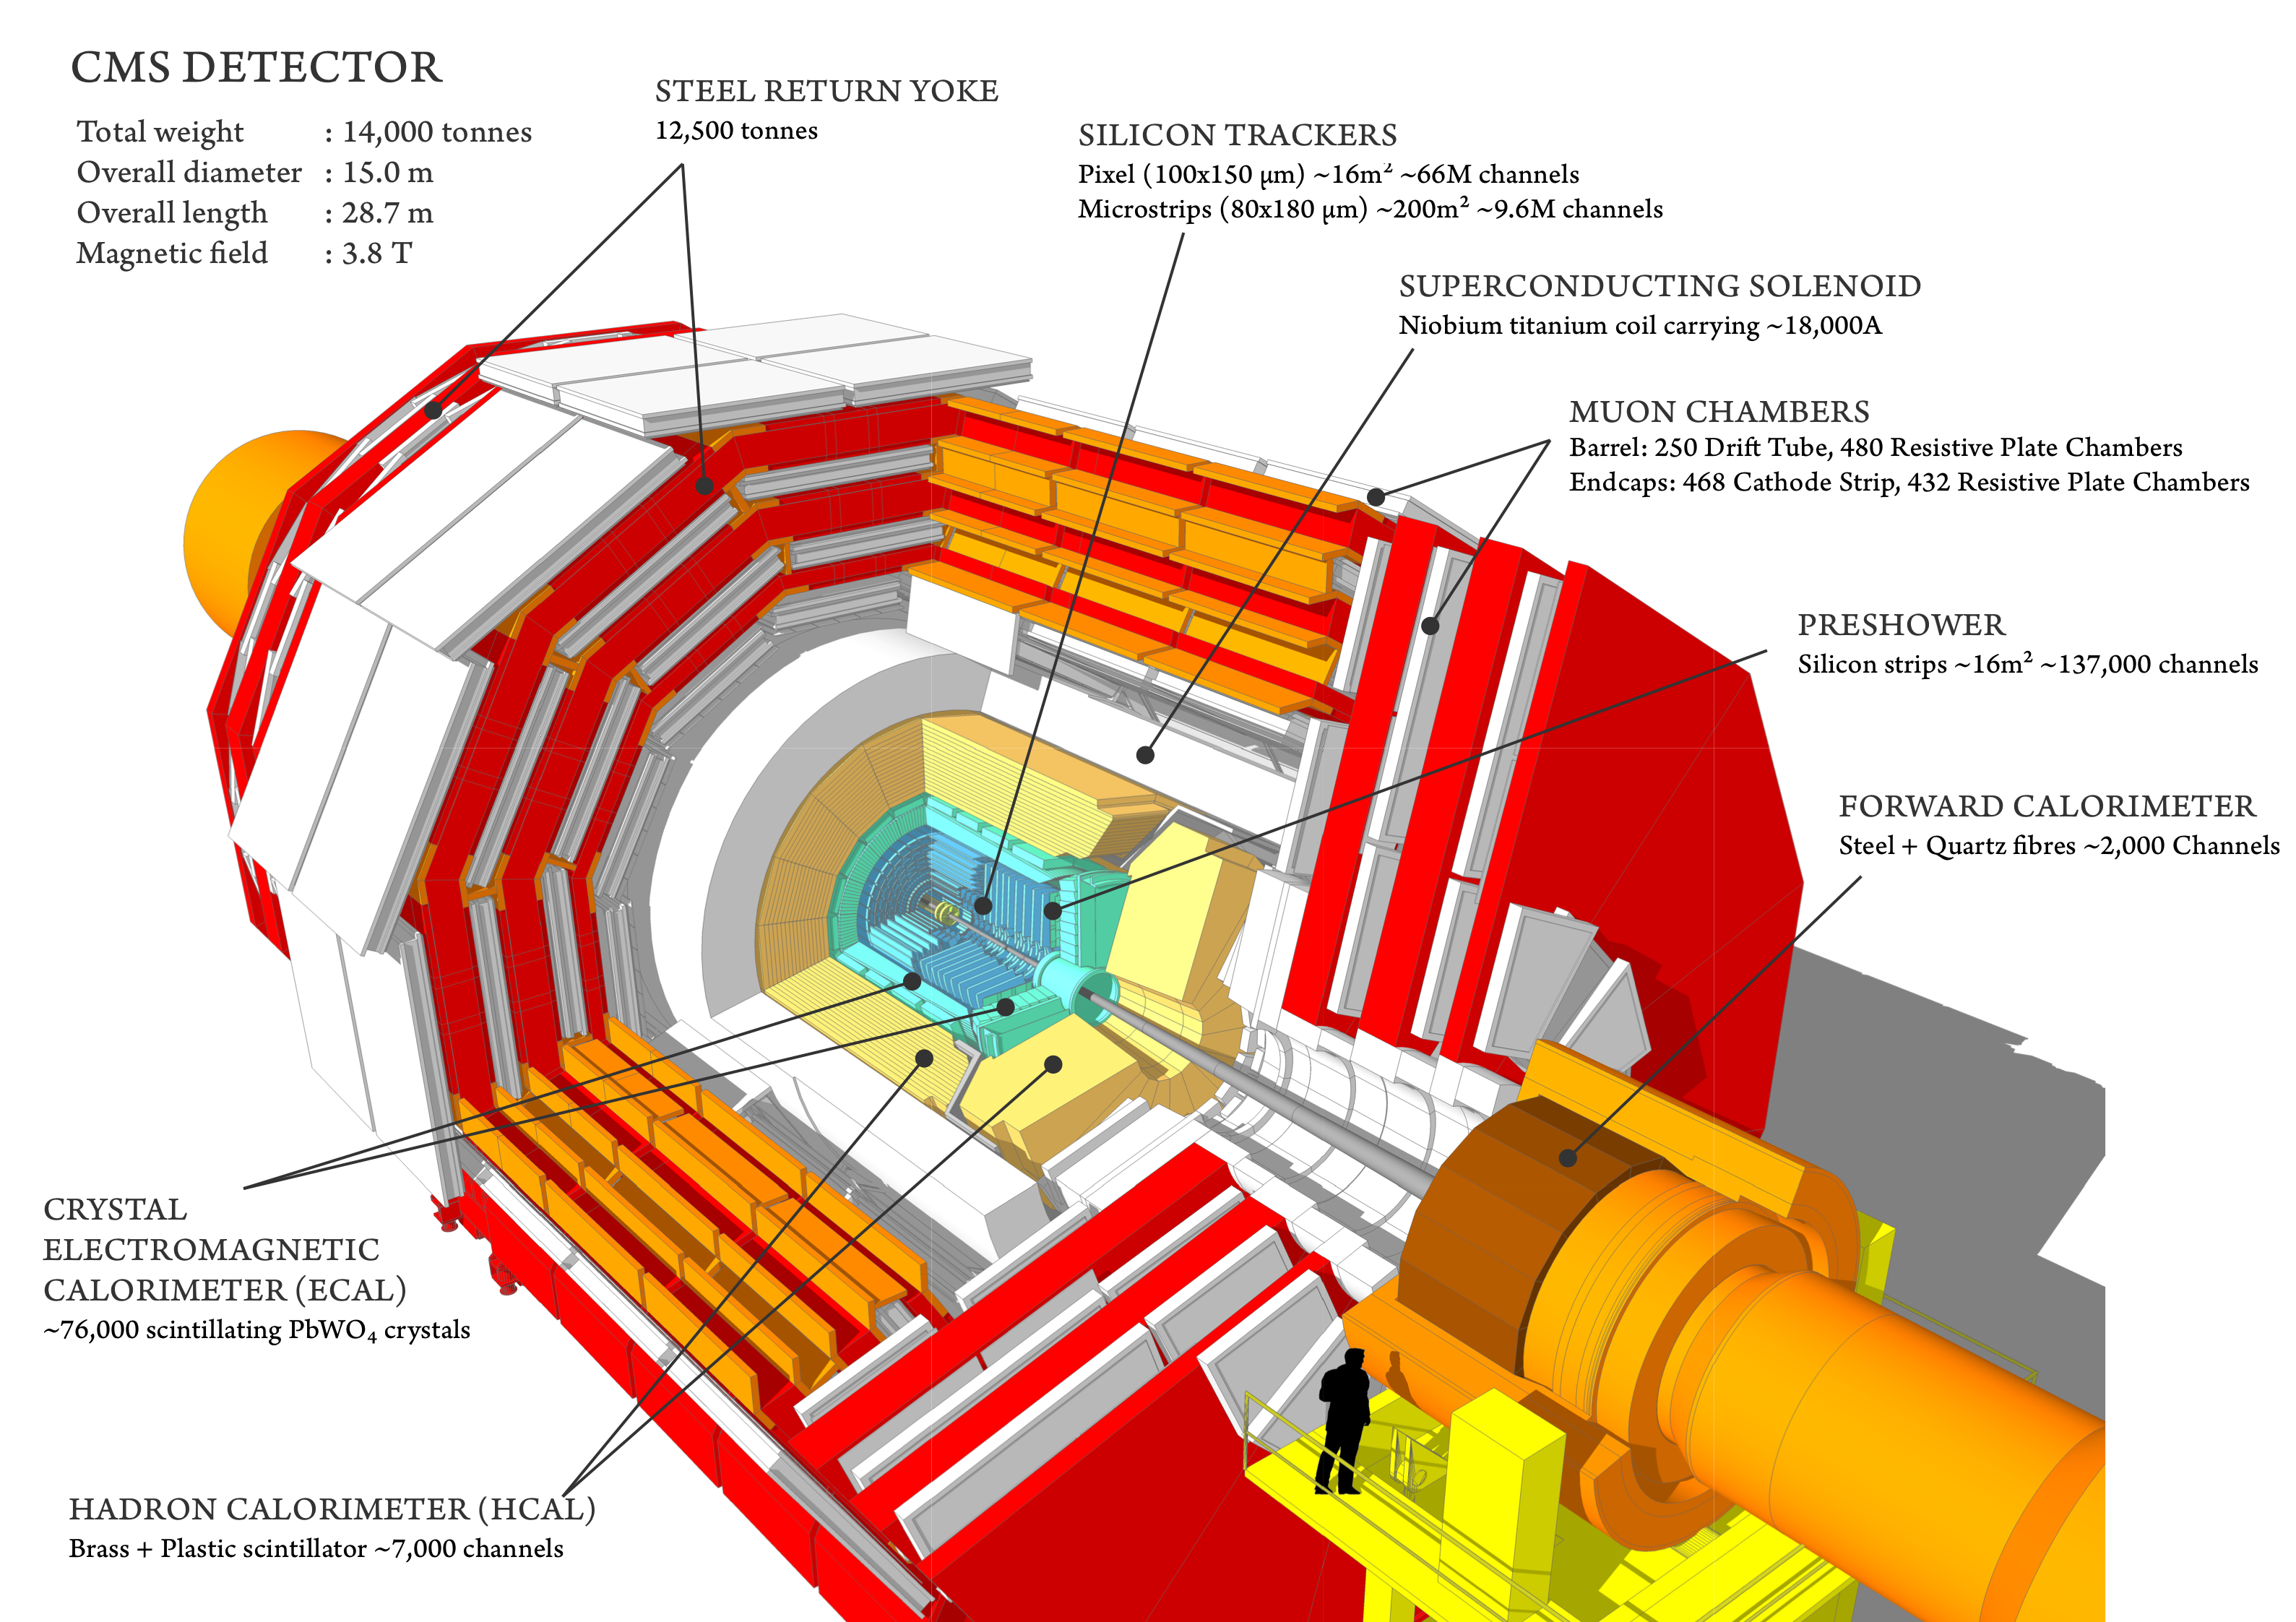
\includegraphics[width=15cm]{F2.png}
\caption{\label{fig:frog} Diseño interno del detector CMS \cite{Bayatian:2006nff}.}
\end{figure}


El solenoide superconductor del experimento CMS tiene 13 m de largo y 6 m de diametro. Es capaz de generar un campo magnético uniforme de 4 T en su interior y está construido por 4 capas de espiras de Niobio-Titanio (NbTi), enfriado a una temoperatura de 4.45K, esto último para que se alcance el estado superconductor. Este solenoide superconductor está rodeado por 5 barriles y 3 discos de hierro, que tienen el objetivo de devolver el campo magnético generando un campo exterior de 2 T.  Esta configuración de campos magnéticos es responsable de curvar las trayectorias de las partículas cargadas.
\\
\\

Dentro del solenoide se encuentra el sistema de reconstrucción de trazas (Tracker System), un sistema de detección diseñado con dos tecnologías: pixeles y tiras de silicio. El tracker system está diseñado para identificar los vértices de las colisiones con una precisión de 9 $\mu$m y una eficiencia del 98\%, esta eficiencia se degrada con el tiempo debido a los daños por radiación que sufren los materiales. Cuando una partícula cargada pasa por este sistema, se crean pares electrón-hueco en el material y esto genera una señal eléctrica que luego es amplificada. Este sistema fue construido para ser bastante resistente a la radiación y se espera que dure 10 años.
\\
\\
Luego de este sistema se encuentra el calorímetro electromagnético (ECAL). Este fue construido para detener electrones y fotones y medir su energía; el sistema está compuesto por cristales de tungstato de plomo, el cual fue escogido por su corta profundidad de radiación, alta densidad y rápido centelleo (25 ns). La única desventaja de este material es su alta sensibilidad de respuesta a la temperatura (2\%/C). Los cristales van perdiendo transparencia con la luminosidad integrada (que es la razón entre la cantidad de eventos o colisiones que se han dado en el LHC y la sección eficaz de colisión para los protones\cite{RuizAlvarez:2016mhn}). Por tanto la transparencia de los cristales tiene que ser corregida constantemente por un sistema de láser. El ECAL cuenta con 61200 cristales en el barril y 7324 en las tapas del calorímetro.
\\
\\
Cuando se colisionan dos partículas constituidas por quarks (hadrones), como los protones en el caso del LHC, se pueden generar quarks en los estados finales de la colisión. Sin embargo, debido al confinamiento del color estos quarks empiezan a agruparse y a formar de nuevo hadrones. Esto puede suceder iterativamente generando ``lluvias de hadrones'' o tambien llamados jets.
\\
\\
Para detener y detectar los jets hadrónicos se diseñó el calorímetro hadrónico (HCAL), cierta parte de este sistema se encuentra dentro del solenoide (Hadron Endcap Calorimeter y Hadron Barrel Calorimeter) y fuera están el Outer Calorimeter y el Hadron Forward Calorimeter (estos permiten extender el rango angular de detección). Los calorímetros tienen el objetivo de detectar los hadrones y lo hacen de la siguiente manera: el sistema tiene intercalados placas de acero con cristales centelladores, las placas de acero generan las cascadas de hadrones y cuando estos pasan por los centelladores, la luz generada es convertida en corrientes eléctricas por fotodiodos híbridos (HPDs). Estas corrientes permiten medir la energía de los hadrones. Es importante mencionar que debido a la posición del Forward Calorimeter, este recibe más radiación comparado con los otros calorímetros hadrónicos. Esto es debido a que el Forward Calorimeter está en la dirección del haz incidente, por tanto, los centelladores fueron construidos de un material más resistente a la radiación como lo es el cuarzo.
\\
\\
Finalmente en la parte más externa del detector están ubicados los detectores de muones, esto se debe a que estas partículas tienen un gran poder de penetración. Las cámaras de detección están hechas de 3 tecnologías diferentes: Drift Tube Chambers (DT), Cathode Strip Chambers(CSC) y Resistive Plate Chambers (RPC). Las 3 están basadas en la detección por ionización de gases: al paso de partículas cargadas se generan corrientes de deriva. En la figura 3 se muestra una recreación a un corte transversal del detector.

\begin{figure}
\centering
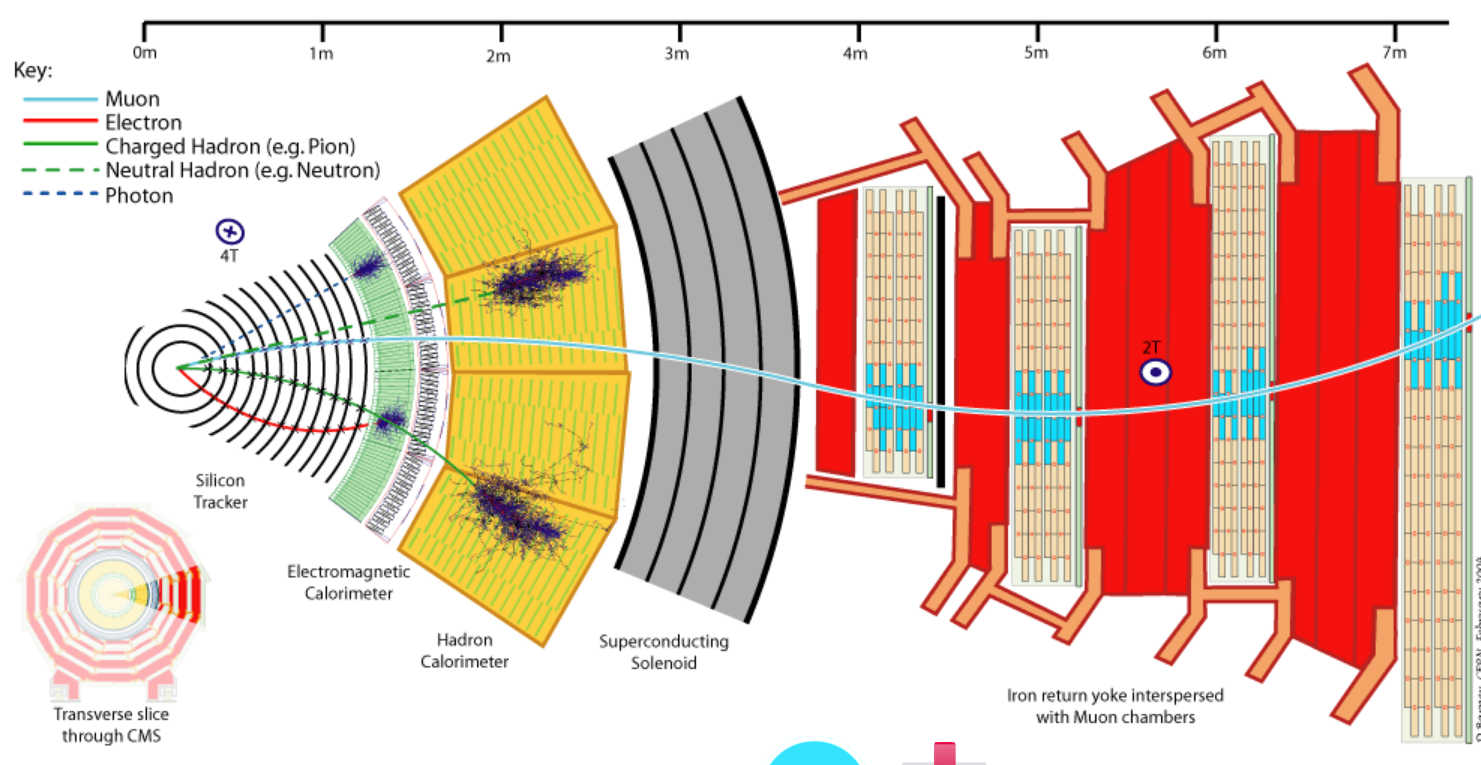
\includegraphics[width=15cm]{F3.png}
\caption{\label{fig:frog} Corte transversal del detector CMS \cite{Bayatian:2006nff}.}
\end{figure}

\subsection{Sistema de Trigger}

CMS fue diseñado para tomar los datos de cada colisión que ocurre	, cada una está separada en el tiempo por 25 ns, esto produce un flujo de datos de 1 PB/s (PB=Petabyte). Por tanto, debe hacerse una selección de eventos en tiempo real, el sistema encargado de hacer esto recibe el nombre de Trigger System y lleva a cabo esta tarea en dos fases \cite{CMSTrigger}. 
\\
\\
La primera de fase es el Level 1 Trigger (L1), este es un proceso basado en Hardware construido específicamente para analizar los datos provenientes de los sistemas de detección y escoger los eventos más interesantes: aquellos que contienen partículas con gran momento transverso o por ejemplo con combinaciones raras de estados finales. Este filtro reduce el flujo de datos en dos ordenes de magnitud y dispone de 3.2 $\mu$s para decidir, esto hace que la memoria de almacenamiento tenga que ser suficiente para guardar los datos de 128  colisiones.
\\
\\
La segunda fase de la selección se conoce como High Level Trigger (HLT). Es un proceso basado en software: una serie de algoritmos corren en granjas de varios miles de procesadores, estos códigos han sido previamente implementados con el objetivo de realizar búsquedas predeterminadas y analizan los datos que salen de L1. El tiempo de decisión de este sistema es de aproximadamente 100 ms y al finalizar la selección, el flujo original de datos ha sido reducido por un factor de cinco ordenes de magnitud.

\subsection{Materia oscura en colisionadores.}

El modelo estándar de la cosmología predice que sólo conocemos como se comporta el 5\% del contenido de materia del universo (materia bariónica), el restante 95\% se cree es: materia oscura (26\%) y energía oscura (69\%) \cite{Ade:2015xua}. Las evidencias indirectas de la existencia de materia oscura son variadas y contundentes: lentes gravitacionales, el cúmulo bala, la radiación cósmica de fondo y la estababilidad del gas caliente en clusters de galaxias son algunas de ellas \cite{Freese:2017idy}. 
\\
\\
Hace 20 años algunas propuestas a candidatos de materia oscura incluían los MACHOS (MAssive Compact Halo ObjectS), que consisten de objetos astrofísicos muy tenues para ser detectados, por ejemplo: agujeros negros, estrellas de neutrones, enanas blancas, etc. Sin embargo, experimentos recientes descartan esta posibilidad y por tanto nos dejan solo con los candidatos no bariónicos como posibles explicaciones \cite{Freese:1999ge,Fields:1999ar}.
\\
\\
Los candidatos más populares actualmente son los WIMPS (Weakly Interacting Massive ParticleS) y los Axiones. Ambas son partículas que surgen como propuesta de solución a otros problemas en física de partículas: Supersimetría (SUSY) \cite{SUSY} y simetría Carga-Paridad en interacciones fuertes (Strong CP) \cite{StrongCP}, respectivamente, y por esto son tan populares. Se sabe que la materia oscura no puede ser caliente, es decir, tener velocidades relativistas, debido a que esto implicaría que el universo debería ser más homogéneo de lo que es. Y tampoco puede interactuar eléctricamente, ya que interaccionaría con el gas interestelar. 
\\
\\
Otros candidatos para materia oscura surgen de modelos más sencillos como el modelo del doblete inerte y pueden ser detectados en aceleradores como muestran recientes trabajos [7,8]. Esta búsqueda en particular se basa en la fusión de bosones vectoriales (VBF) ya que el candidato a materia oscura $H^0$ tiene carga débil. En la figura 4 podemos ver los procesos que contribuyen en este tipo de busquedas, como vemos de los estados finales en los diagramas (jets que se detectan y el candidato de materia oscura escapa), las busquedas se basan en energía transversa faltante (MET) asociada a procesos con dos jets con energía transversa $E_T$ alta y detectados en hemisferios diferentes.
\begin{figure}
	\centering
	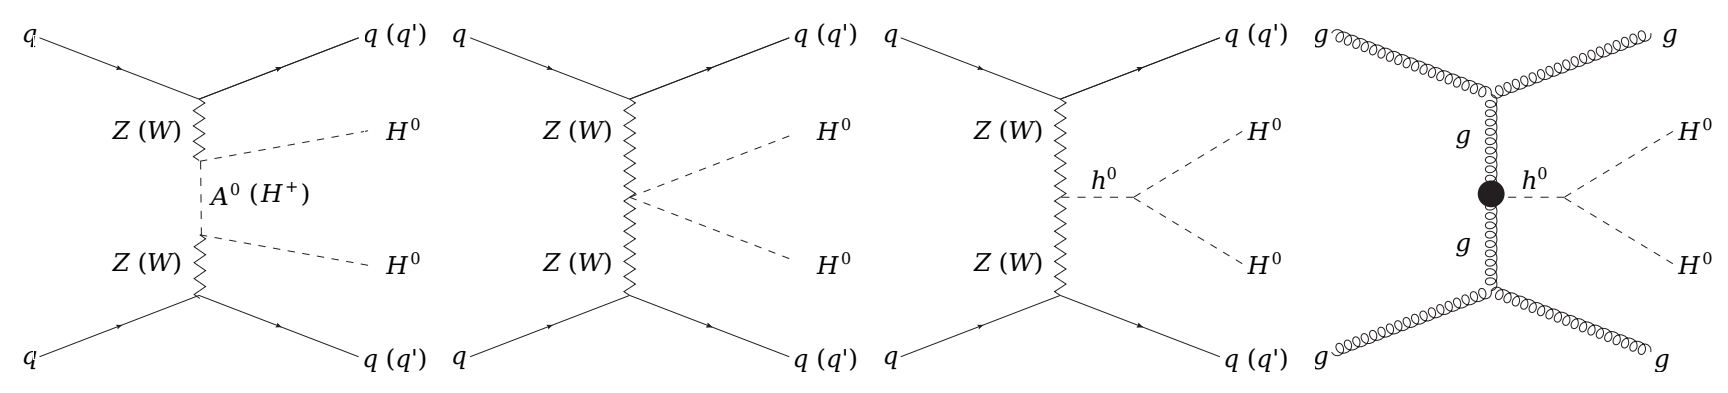
\includegraphics[width=15cm]{F4.png}
	\caption{\label{fig:frog} Diagramas de Feynman que contribuyen a pp$\rightarrow H^0H^0 jj$. El punto en la cuarta figura denota el acople entre el Higgs del modelo estándar y los gluones.}
\end{figure}
\\
\\
Las búsquedas en aceleradores como el LHC se basan en el rastreo de estados finales de partículas del modelo estándar con energía transversa faltante [7], de esta manera sabríamos que la partícula de materia oscura vivió lo suficiente como para escapar del detector sin decaer, sin embargo esto no dejaría claro que tan estable es la misma para ser materia oscura y por tanto es necesario complementar la información con experimentos astrofísicos. [9]
\newpage
\section{Problema y pregunta de investigación}

	Conforme a lo establecido en las secciones anteriores, podemos ver que el problema de encontrar la materia oscura debe resolverse, en parte, mediante la busqueda de la misma en colisionadores. Ya hemos visto que modelos como [7,8] motivan busquedas en experimentos como LHC, sin embargo, debido a la cantidad de datos que toman detectores como CMS se deben idear filtros que nos dejen con la información que consideramos relevante a la hora de realizar las búsquedas, por tanto nuestra idea es responder: \textbf{¿Qué Hight Level Trigger para el experimento CMS del CERN con muones de bajo $p_T$ (monento transverso) es pertinente para su uso en el estudio de señales de materia oscura en el detector?}


\newpage
\section{Objetivos y cronograma}


\subsection{Objetivo general}

Desarrollar y validar un path Hight Level Trigger (HLT) para el experimento CMS del CERN pertinente para su uso en el estudio de señales de materia oscura con muones de bajo $p_T$ en el detector.

\subsection{Objetivos específicos}

\begin{itemize}
	\item Estudio del modelo que desea ponerse a prueba, estudiando la señal que quiere detectarse y sus backgrounds.
	\item Construcción de un path del HLT usando la herramienta de CMS.
	\item Estudiar la eficiencia y otras características de dicho path del HLT y proponerlo.
	\item Aplicar el HLT al menos a un modelo específico, un ejemplo podrían ser los modelos [7,8].
\end{itemize}


\subsection{Cronograma.}

\begin{table}[h]
	\centering
	\resizebox{\textwidth}{!}{%
	
	\begin{tabular}{|c|c|c|c|c|c|c|c|c|}
		\hline
		Trimestre                              & 2017-3 & 2017-4 & 2018-1 & 2018-2 & 2018-3 & 2018-4 & 2019-1 & 2019-2 \\ \hline
		Revisión de bibliografía.              & *      & *      & *      & *      & *      & *      & *      &        \\ \hline
		Estudio herramienta HLT de CMS.        &        & *      & *      & *      &        &        &        &        \\ \hline
		Estudio fenomenológico.                &        &        & *      & *      &        &        &        &        \\ \hline
		Construcción del HLT                   &        &        &        & *      & *      & *      &        &        \\ \hline
		Estudio de eficiencia.                 &        &        &        &        & *      & *      &        &        \\ \hline
		Aplicar el HLT a un modelo específico. &        &        &        &        &        & *      & *      &        \\ \hline
		Redacción tesis.                       &        &        &        &        &        &        & *      & *      \\ \hline
	\end{tabular}
}
\end{table}

\newpage

\section{Infraestructura y recursos.}

\textbf{Recursos computacionales.}

Para utilizar las herramientas de simulación de eventos como MADGRAPH, PYTHIA y DELPHES se necesita acceso a un cluster computacional de mediana capacidad	 50 núcleos y 1 TB de almacenamiento. Para el procesamiento de datos provenientes de LHC se necesita acceso a la red computucional de CERN (grid) y esto solo es posible si se es miembro.

\newpage


\vspace{0.5cm}

[7] Vector Boson Fusion in the Inert Doublet Model, Bhaskar Dutta, Guillermo Palacio, Diego Restrepo, José D. Ruiz.

\vspace{0.5cm}

[8] Andres G. Delannoy et al., “Probing Dark Matter at the LHC using Vector Boson Fusion
Processes,” Phys. Rev. Lett. 111, 061801 (2013).

\vspace{0.5cm}

[9] Review of Dark Matter searches at colliders, Sarah Alam Malik.

\bibliography{biblibo}
\bibliographystyle{ieeetr}
\end{document}